% -*-coding: utf-8 -*-

\defaultfont

\BiChapter{模板选择及使用中的一些技巧}{Some Tricks of Using this Template}
\label{Tricks}

\BiSection{关于学位论文模板}{Something About Templates}
\label{tricks:abouttemplates}

大家都会有这样的疑问:
我是自己写论文排版,还是使用学位论文模板直接套用格式?
如果要使用模板,我该使用那种模板,Word 还是~\LaTeX 模板?

对于这样的问题,每个人根据自己的情况,可以做出不同的选择,各种工具,萝卜白菜,各有所爱而已。
这里不会非让你采用此模板不可,仅仅给出一些尽量客观的说明供参考。
最后敬请注意,这是一家之言。:-)

\BiSubsection{有没有必要使用模板?}{Necessary to Use Templates?}
\label{tricks:necessaryornot}

研究生院版面上~2005 年~7 月左右有过一场很热烈的争论,话题是研究生院是否要出台官方模板。
这个话题的挑起缘由是:部分网友感觉学校的学位论文规范不详细,导致打印了好几次论文,
反复调整格式,浪费了很多时间、精力和金钱。一位研究生院老师和少数同学从个人角度出发,
认为学校没有必要出台论文模板,也不支持,因为学生写作学位论文的过程中应该学会使用软件
进行排版。然而更多同学认为在时间很紧的情况下,根本没有时间投入大量的精力去按照论文规范
来调整论文的格式,应该使用模板,把更多的时间投入到论文内容的完善中去,因为即便是大家常用的 word 软件,完全从零开始,做出一个完全符合工大论文规范的学位论文样式就要耗费大量的时间,
没有必要大家都来做这个重复性的工作,只要能够会用模板达到学校的格式要求就可以了。
话题讨论两三天后的结果是:官方没有正式回复,不了了之。争论过程可以通过下面的链接
详细了解:~\href{http://bbs.hit.edu.cn/cgi-bin/bbs/bbs0an?path=\%2Fgroups\%2FGROUP\%5F6\%2FTeX\%2Ftex05\%2Fabout}{论文规范完整性及模板必要性讨论}。

本模板作者们和大多数同学的观点一致,所以坚持了此模板的维护,
并且经过多人的继续精心完善,LaTeX 模板越来越成熟完善,消除了所有发现的问题。

不知道你是如何看待这个问题的,你会选择模板么? 如果你选择了``不'',那么下面介绍模板的内容你可以忽略,关闭此文档了。:)

\BiSubsection{我该选择哪个模板?}{Which Templates I should Select?}
现在校内有两类软件做的模板:word 和~ LaTeX。

需要提醒的是,别管用哪个模板,都请了解一下\href{http://hitgs.hit.edu.cn/}{研究生院}出台的官方学位论文规范。:)
在本模板的~ ThesisCriterion 目录下提供了一份论文规范,方便用户使用。

下面分别对两类模板做一简单介绍。

\BiSubsubsection{Word模板}{Word Templates} 现在校内流行的~ word 模板
最初是~ Sun@hit 几年前做的,后来也经一些同学完善,校内~ ftp
可以下载到的是~ 2004 年 的修改版,在
~\href{ftp://202.118.224.241/study/\%C6\%E4\%CB\%FB\%D7\%CA\%C1\%CF/\%C2\%DB\%CE\%C4\%C4\%A3\%B0\%E6}{ftp://202.118.224.241/study/其他资料/论文模版}
里有一份。这个模板,实现了论文规范的章节标题、目录等样式要求,基本满足了学位论文写作的需要,
但是没有包括博士论文要求的中英文目录同时生成的方法,
对使用方法介绍比较简略,而且没有及时把研究生院的最新论文规范修改添加进去,还请注意。

如果使用这个模板来写论文,请先了解一下~ word 写大论文的技巧,包括样式的使用,目录的更新,图表的自动编号的实现,参考文献的编号和排序,
交叉引用,书签生成等方法。 推荐台湾同胞侯捷写的书籍《word排版艺术》,这是目前写得最好的一本~ word 教程了,
对这些技巧介绍比较详细,还介绍了一些排版的基本常识。

若使用~ Word 模板,请经常注意备份文档(最好是别的机器上或者电子信箱保存),
尽量别中途更换~ word 版本,避免格式变化或者文档损坏,最后注意保持杀毒软件实时监控,
防止感染针对~word 文档的病毒。

最后,打印纸本的时侯,最好转化成~PDF 进行打印,防止在其他机器上格式改变。另外,一些同学体验是~ PDF 文件打印的效果要好于~ word 直接打印。

如果你用了上面的几点注意事项,可以减少你用~ word 排版论文的繁杂过程,事半功倍。

\BiSubsubsection{LaTeX模板}{LaTeX Templates}
校内的~ LaTeX
研究生论文模板目前有三个:数学系已毕业的一位同学赵安国做的早期的本硕博学位论文文档类,
pineapple@hit
正在完善的初具雏形的本硕博文档类,还有本模板(硕博士模板,不包含本科)。前两者
都是标准的文档类,条理较清晰,不过第一个模板现在无人维护,而第二个目前还不完善,
很多细节需要调整。 本模板采用的是~ LaTeX 已有的~ book
文档类上修改的方式,需要调整的内容分散在各个文件中,条理性相对差了一下,
不过与前两者相比,由于使用的基本上都是~ LaTeX 常用命令,一般用户上手修改很容易完成,
自己的论文内容管理也不算麻烦,而且功能更完善,
目前用户及参与维护者较多,所以这里推荐采用本模板。

后面的章节将详细介绍本模板的使用方法技巧,这里简单介绍一下本模板的几点特色:
\begin{itemize}
  \item 由于~ LaTeX 系统的跨平台性,可运行于~ Windows、Linux、Mac 等操作系统;
  \item 由于~ LaTeX 系统本身的安全性,不会出现不稳定、中病毒及文件损坏的现象;
  \item 由于 ~LaTeX 系统不同于~ MSWord 的所想即所得的排版方式,可以更专注于论文内容;
  \item 由于~ LaTeX 模板的易用自动性,完全不用自己手动调整论文格式;
  \item 格式已经完全定制,只需在源文件中填充自己的内容,完全不用考虑论文格式问题;
  \item 论文封面、中英文目录、中英文图表目录(包括子图)、书签同时自动生成;
  \item 公式、图形、表格、参考文献等自动编号、交叉引用方便;
  \item 生成 ~PDF 格式论文,专业、漂亮;
  \item 紫丁香 ~TeX 版提供使用及维护支持。
\end{itemize}

通过前面的介绍,你也了解了一些~LaTeX 的特点,和你对~word 的认识对比,你该选择哪个模板呢?
如果你选择了 ~word 模板,那么你也可以关闭此文档了。 :-)

\BiSection{本模板有关说明}{Readme}
\BiSubsection{软件环境}{Environment of Software}
该模板在~\LaTeX{}+CJK 环境下均可正常编译,但在某些的软件环境下可能会遇到一
些编译问题,因此建议使用我们推荐的软件环境:
\begin{hitlist}
\item WindowsNT/2000/XP+CTeX:CTeX 是目前国内影响力最大的中文~TeX 社区,CTeX
软件安装方便,集成了大多数常用的软件,如果不想考虑太多软件本身的问题
而只想专注于论文的话,CTeX 是个不错的选择,http://www.ctex.org 是~ CTeX 的主
页,在这里可以获得最新的消息、关于~TeX 的帮助~(CTeX
论坛)和最新的软件;需要说明的是,CTeX 2.4 基于 miktex 2.4,支持PlutoThesis的dvipspdf,dvipdfmx和pdflatex的中文处理方式,不支持xelatex 字体处理方式,还请注意。
\item WindowsNT/2000/XP/vista+MiCTeX:由于 ctex 套装在最近的两三年内没有更新,仍然是基于MikTeX2.4版,而MiKTeX 2.5版之前都已不再维护,目前最新为2.7版,具有不少新特性,尤其是 直接利用系统字体的XeTeX的字体处理方式和对vista的良好支持。所以 instanton@ctex 在MiKTeX 2.7的基础上加上了dvipspdf,dvipdfmx和pdflatex中文处理,发布了 MiCTeX,可以在ctex论坛上找到发布和下载信息,241 ftp上可能也有不保证最新的版本下载。 MiCTeX配置的编辑器是scite,对于新手来说不如winedt好用,可以在安装 mictex后直接安装winedt做为编辑器,无需额外配置;
\item windows2000/XP/vista+MiKTeX:若是用户只是用xelatex处理中文,或者是只处理英文文档,可以考虑安装MiKTeX最新版;
\item Linux+TeXlive:TeXlive 是一个著名的~ TeX 发行版,支持众多的操作系统,
但是没有对中文的直接支持,需要自行配置字体;请关注ctex论文,tex@newsmth和241 ftp去获取最新的版本。
\end{hitlist}

以上软件环境均经过测试,可以正常编译该模板,在其它软件环境下可能遇到的
问题是缺少中文字体或缺少宏包,如果遇到相应问题,欢迎到紫丁香~BBS 的~TeX 版
讨论。


\BiSubsection{相关目录及文件}{The Related Directories and Files}
表~\ref{Introduction:Tab1}给出了与模板相关的目录和文件的说明。建议首先了解这些文件的用途,把握论文模板的结构框架,
然后打开各个文件,查看注释和一些命令,更详细的了解,为使用打下良好基础。

一般用户在写作过程中只需关注~\ref{Introduction:Tab1}中前六项内容,即~main.tex, preface, body, appendix,
figures, reference,后面几项无需改动。从~1.8~正式版开始,进行模板升级时,一般只要把~setup 目录,
chinesebst.bst, gb\_452.cap, gb\_452.cpx, Authorization.tex 替换掉即可。

\begin{table}[htb]
\centering 
\TableBiCaption{模板目录和文件说明}{Description of Directories and Files}
\label{Introduction:Tab1}
\begin{tabular}{lp{11cm}}
\specialrule{1.4pt}{-2pt}{2pt}%\hline\hline
main.tex    & 主文件,如不需要图表索引,在此文件中注释掉\\
preface     & 前言部分,包括封面,中文摘要,英文摘要,主要符号表等\\
body        & 正文部分,包括正文各章节和结论\\
appendix    & 附录部分,包括致谢,附录章节和个人简历及发表的文章列表等\\
figures     & 存放所有插图的目录\\
reference   & 存放参考文献.bib 文件的目录,bib 文件可以从~scholar.google~下载\\
setup       & 存放设置文件的目录,其中package.tex 包含对宏包的引
              用和参数设置;format.tex 包含具体的格式调整和定义;
              Definition.tex 包含另外一些相关的定义;figtab.tex
              是图表索引;type.tex是硕博类型分类,以上这些用户一般无需改动。\\
readme.pdf  & 一个编译后得到的完整论文示例及论文模板使用及更新说明 \\
make.bat    & 在~Windows下自动选用~dvips 、~dvipdfm、~pdfLaTeX、xelatex 完整编译和自动清理无用文件的脚本文件
              ,建议了解其中命令\\
clean.bat   & 用来删除所有编辑和编译时产生的临时文件,pdf 文件除外\\
chinesebst.bst & 生成包括中文参考文献的标准形式的定义文件\\
makefile    & linux下用来自动编译和清除无用的文件\\
gb\_452.cap & aloft的gb.cap的4.5.2版,包含了中文格式有关的基本定义。
              BaconChina对原始版本进行了少量修改,所以请勿用其它版本覆盖\\
gb\_452.cpx & 与gb\_452.cap 内容完全一样的文件。不同的\LaTeX 系统要求
              不同的文件后缀,两个文件保证了兼容性\\
\specialrule{1pt}{0pt}{0pt}%
\end{tabular}
\end{table}


\BiSubsection{论文最新模板下载及更新方法}{Downloading and Updating Methods of Updated Template Downloading and Updating Methods of Updated Template Downloading and Updating Methods of Updated Template}
\BiSubsubsection{论文模板下载}{Template Downloading Method}
哈尔滨工业大学~ PlutoThesis 硕博士学位论文模板的维护站点是~\url{http://gf.cs.hit.edu.cn/projects/plutothesis/} 或者 ~\url{http://code.google.com/p/plutothesis/},
从这里的``文件'' 页(~\url{http://gf.cs.hit.edu.cn/frs/?group_id=91})或者 ~\url{http://code.google.com/p/plutothesis/downloads/list} ~可以下载到发布的所有模板,
并且察看每个发布版本的更新日志,加深对模板的了解(当然,您也可以下载最新的模板,然后看其中的readme.pdf,更详细)。
建议采用最新的模板,因为最新的模板消除了已发现的一些使用或与论文规范不完全吻合的~bugs,在使用上也可能更方便一些。\textcolor{red}{在您完成论文准备打印或者提交正式稿之前,请到本站来检查一下您所使用的版本是否是本模板的最新版本,以保证您的论文能够完全符合研究生院的论文格式要求。}

对于未发布版本(正在维护的版本,可能已经修复了部分bug,可能某些bug还没有解决),如果您想了解,
建议使用版本控制系统~subversion 的客户端访问版本库,访问方法是~\url{https://svn.gf.cs.hit.edu.cn/svn/plutothesis/} 或 ~\url{http://code.google.com/p/plutothesis/source/checkout} 上查看说明,并下载你感兴趣的版本。
subversion 介绍及使用介绍的网站很多,你可以通过~google 搜索。
个人推荐~ \url{http://www.subversion.org.cn},有一些不错的教程,论坛上也有一些高手。
Windows 下最好用的~svn 客户端是~tortoisesvn,和资源管理器结合很紧密,右键菜单操作,很方便;linux 下比较好用的是~rapidsvn。

\BiSubsubsection{论文模板更新方法}{Template Updating Method}
从~1.8rc2~开始,进行模板升级时,一般只要把~setup 目录,
chinesebst.bst, gb\_452.cap, gb\_452.cpx, Authorization.tex 替换掉即可
个人建议论文写作最好采用~Subversion 进行版本控制,从而做好备份工作,也方便版本管理,顺利完成论文撰写工作。
对于您在论文写作过程中用到的程序,最好也同时进行版本控制。这是一个很好的写作和编程习惯。

\BiSection{模板技巧介绍}{Tricks Introduction}
\label{Tricks:Introduction}
在使用本模板之前,你已经具备看懂本模板中一些用户需要使用的命令的能力,最好是找一个模板,
把你的一篇~article 排版一遍。\LaTeX~的基本概念、命令和操作请参考~TeX 版置底里推荐的相关资料。
本节往后简单介绍使用本模板的一些技巧。

\BiSection{硕博士论文选项}{Doctor or Master Thesis}

使用模板,选择按硕士还是博士论文格式,在 main.tex 如下的命令里控制, 把不符合你要求的选项注释掉就可以了。
博士学位论文只要求双面打印,硕士学位论文可以选择单面还是双面打印,双面打印时页眉不同。\vspace{-5pt}
\begin{verbatim}
    %\def \xuewei {Doctor}   % 定义学位 博士
    \def \xuewei {Master}    % 硕士
    \def\oneortwoside{oneside} %定义单双面打印,只针对硕士学位论文进行单面打印有效;
    %\def\oneortwoside{twoside} % 硕士双面打印
\end{verbatim}

下面选择你所属的学科:\vspace{-5pt}
\begin{verbatim}
    \def \xueke {Engineering} % 定义学科 工学
    %\def\xueke{Science}      % 理学
    %\def\xueke{Management}   % 管理学
    %\def\xueke{Arts}         % 艺术学
\end{verbatim}

选择论文的编译方式:\vspace{-5pt}
\begin{verbatim}
    \def\usewhat{dvipdfmx}    % 你喜欢哪种编译方式,pdflatex dvipdfmx dvipspdf xelatex yap
\end{verbatim}
无论选择哪一个,只要运行~make.bat 脚本,就会自动按照你选择的方式进行完整编译,生成最终文件。

采用pdflatex, dvipdfmx, dvipspdf编译时,由于latex没有times new roman字体,所以只能用times宏包仿times new roman,得到的pdf文件中不是真正的times new roman字体。而用xelatex可以直接调用系统的times new roman字体。

需要着重指出的是,本模板采用GBK编码,若选用xelatex编译,在含有参考文献的情况下,需在bibtex生成的bbl文件中头文件处指明编码,目前系统不能自动生成此编码说明,从而导致参考文献乱码。使用make.bat编译时,已经用fixbbl.txt和bbl文件进行合并的方式进行了自动修正,生成参考文献正常,所以推荐用make.bat编译,或者是参考make.bat的命令,各取所需。

用户自己的章节文件和图片路径文件,可以通过修改~main.tex 中下列命令的内容实现。\vspace{-5pt}
\begin{verbatim}
  \includeonly、  \include、 \graphicspath
\end{verbatim}

\BiSection{封面内容}{Cover Contents}
封面内容及中英文摘要主要在~ preface/cover.tex 中定义,cover.tex 中已经对相关选项详细注释说明;
封面的格式是在~setup/format.tex 中设置的,一般用户无需修改。


\BiSection{中英文目录}{Chinese and English Contents}
\label{Tricks:Contents}
本文分别为章、节、小节和小小节定义了新命令:

\begin{verb}
\BiChapter、\BiSection、\BiSubsection和\BiSubsubsection
\end{verb}

上述~4 个命令的使用方法如~\verb"\BiChapter{中文标题}{engish}" 和 ~\verb"\BiSection{中文标题}{engish}"所示。
对于章节标题比较长的情况,已经实现在正文和目录中自动换行的功能。

另外,更新过的~\verb"\BiChapter" 还支持在正文中手动换行或自动换行,在目录中自动换行,
使用格式为~\verb"\BiChapter[放到目录中的]{长标题\\手动换行}{english title}"。
对于节及小节,可以仿照~.../setup/definition.tex 中章的形式自己定义类似的设置。不过这种情况很少出现,所以这里没有
再更新定义。如果您需要,JUST DO IT YOURSELF. :-)

对于附录中没有章标号的章,如结论等,也定义了一个相应的命令\verb"\BiAppendixChapter"。

对于附录中有章标号的章,定义了一个相应的命令\verb"\BiAppChapter"。

在这些命令中均含有两个参数,第一个为中文题目,第二个为英文题目。

为了浏览统计查找方便,本模板增加了中英文图表目录,但是哈工大的研究生论文规范中并没有这条要求,
如果您不需要,请到~main.tex 中把这句代码注释掉(文件中已注明)。
\begin{verb}
   % -*-coding: utf-8 -*-

%% 中英文插图、表格、算法索引   
%% 硕博士学位论文规范均不要求这一项,请正式打印的时候在main.tex中屏蔽掉% -*-coding: utf-8 -*-

%% 中英文插图、表格、算法索引   
%% 硕博士学位论文规范均不要求这一项,请正式打印的时候在main.tex中屏蔽掉% -*-coding: utf-8 -*-

%% 中英文插图、表格、算法索引   
%% 硕博士学位论文规范均不要求这一项,请正式打印的时候在main.tex中屏蔽掉\input{figtab.tex};

\ifxueweidoctor
  %\clearpage{\pagestyle{empty}\cleardoublepage}   % 清除目录后面空页的页眉和页脚
\else%
  {\ifoneortwoside\clearpage{\pagestyle{empty}\cleardoublepage}\else\newpage\fi} % 清除目录后面空页的页眉和页脚
\fi

\addcontentsline{toc}{chapter}{\hei 插~~~~图}   % 中文插图加入到中文目录
\listoffigures                                  % 生成中文 图形索引

\ifxueweidoctor                                 %硕士学位论文没有英文目录
%\clearpage{\pagestyle{empty}\cleardoublepage}   % 英文图形索引 右开 ?需要吗?
\pdfbookmark[0]{List of Figures}{listfigure}
\addcontentsline{toe}{chapter}{\bfseries\xiaosi List of Figures} % 英文插图加入到英文目录
\listoffigen                                    % 生成英文图索引
\fi

\ifxueweidoctor
  %\clearpage{\pagestyle{empty}\cleardoublepage}   % 清除目录后面空页的页眉和页脚
\else%
  {\ifoneortwoside\clearpage{\pagestyle{empty}\cleardoublepage}\else\newpage\fi}   % 清除目录后面空页的页眉和页脚
\fi

\addcontentsline{toc}{chapter}{\hei 表~~~~格}   % 中文表格加入到中文目录
\listoftables                                   % 生成中文 表格索引

\ifxueweidoctor                                 %硕士学位论文没有英文目录
  %\clearpage{\pagestyle{empty}\cleardoublepage}   % 英文表格索引 右开 ?需要吗?
  \addcontentsline{toe}{chapter}{\bfseries\xiaosi List of Tables} % 英文表格加入到英文目录
  \pdfbookmark[0]{List of Tables}{listtable}
  \listoftblen                                    % 生成英文 表格索引
\fi
%% 如果不需要图表索引,注释掉上面的即可

\ifxueweidoctor
  %\clearpage{\pagestyle{empty}\cleardoublepage}   % 清除目录后面空页的页眉和页脚
\else%
  {\ifoneortwoside\clearpage{\pagestyle{empty}\cleardoublepage}\else\newpage\fi}   % 清除目录后面空页的页眉和页脚
\fi

\addcontentsline{toc}{chapter}{\hei 算~~~~法}   % 中文算法加入到中文目录
\renewcommand{\listalgorithmcfname}{算~~~~法}   %中文“算法”代替英文list of algorithms
\listofalgorithms                               % 生成中文算法索引

\ifxueweidoctor                                 %硕士学位论文没有英文目录
  %\clearpage{\pagestyle{empty}\cleardoublepage}   % 英文算法索引 右开 ?需要吗?
  \addcontentsline{toe}{chapter}{\bfseries\xiaosi List of Algorithms} % 英文算法加入到英文目录
  \pdfbookmark[0]{List of Algorithms}{listAlgo}
  \listofalgoen                                    % 生成英文 表格索引
\fi


%%% Local Variables: 
%%% mode: latex
%%% TeX-master: "../main"
%%% End: 
;

\ifxueweidoctor
  %\clearpage{\pagestyle{empty}\cleardoublepage}   % 清除目录后面空页的页眉和页脚
\else%
  {\ifoneortwoside\clearpage{\pagestyle{empty}\cleardoublepage}\else\newpage\fi} % 清除目录后面空页的页眉和页脚
\fi

\addcontentsline{toc}{chapter}{\hei 插~~~~图}   % 中文插图加入到中文目录
\listoffigures                                  % 生成中文 图形索引

\ifxueweidoctor                                 %硕士学位论文没有英文目录
%\clearpage{\pagestyle{empty}\cleardoublepage}   % 英文图形索引 右开 ?需要吗?
\pdfbookmark[0]{List of Figures}{listfigure}
\addcontentsline{toe}{chapter}{\bfseries\xiaosi List of Figures} % 英文插图加入到英文目录
\listoffigen                                    % 生成英文图索引
\fi

\ifxueweidoctor
  %\clearpage{\pagestyle{empty}\cleardoublepage}   % 清除目录后面空页的页眉和页脚
\else%
  {\ifoneortwoside\clearpage{\pagestyle{empty}\cleardoublepage}\else\newpage\fi}   % 清除目录后面空页的页眉和页脚
\fi

\addcontentsline{toc}{chapter}{\hei 表~~~~格}   % 中文表格加入到中文目录
\listoftables                                   % 生成中文 表格索引

\ifxueweidoctor                                 %硕士学位论文没有英文目录
  %\clearpage{\pagestyle{empty}\cleardoublepage}   % 英文表格索引 右开 ?需要吗?
  \addcontentsline{toe}{chapter}{\bfseries\xiaosi List of Tables} % 英文表格加入到英文目录
  \pdfbookmark[0]{List of Tables}{listtable}
  \listoftblen                                    % 生成英文 表格索引
\fi
%% 如果不需要图表索引,注释掉上面的即可

\ifxueweidoctor
  %\clearpage{\pagestyle{empty}\cleardoublepage}   % 清除目录后面空页的页眉和页脚
\else%
  {\ifoneortwoside\clearpage{\pagestyle{empty}\cleardoublepage}\else\newpage\fi}   % 清除目录后面空页的页眉和页脚
\fi

\addcontentsline{toc}{chapter}{\hei 算~~~~法}   % 中文算法加入到中文目录
\renewcommand{\listalgorithmcfname}{算~~~~法}   %中文“算法”代替英文list of algorithms
\listofalgorithms                               % 生成中文算法索引

\ifxueweidoctor                                 %硕士学位论文没有英文目录
  %\clearpage{\pagestyle{empty}\cleardoublepage}   % 英文算法索引 右开 ?需要吗?
  \addcontentsline{toe}{chapter}{\bfseries\xiaosi List of Algorithms} % 英文算法加入到英文目录
  \pdfbookmark[0]{List of Algorithms}{listAlgo}
  \listofalgoen                                    % 生成英文 表格索引
\fi


%%% Local Variables: 
%%% mode: latex
%%% TeX-master: "../main"
%%% End: 
;

\ifxueweidoctor
  %\clearpage{\pagestyle{empty}\cleardoublepage}   % 清除目录后面空页的页眉和页脚
\else%
  {\ifoneortwoside\clearpage{\pagestyle{empty}\cleardoublepage}\else\newpage\fi} % 清除目录后面空页的页眉和页脚
\fi

\addcontentsline{toc}{chapter}{\hei 插~~~~图}   % 中文插图加入到中文目录
\listoffigures                                  % 生成中文 图形索引

\ifxueweidoctor                                 %硕士学位论文没有英文目录
%\clearpage{\pagestyle{empty}\cleardoublepage}   % 英文图形索引 右开 ?需要吗?
\pdfbookmark[0]{List of Figures}{listfigure}
\addcontentsline{toe}{chapter}{\bfseries\xiaosi List of Figures} % 英文插图加入到英文目录
\listoffigen                                    % 生成英文图索引
\fi

\ifxueweidoctor
  %\clearpage{\pagestyle{empty}\cleardoublepage}   % 清除目录后面空页的页眉和页脚
\else%
  {\ifoneortwoside\clearpage{\pagestyle{empty}\cleardoublepage}\else\newpage\fi}   % 清除目录后面空页的页眉和页脚
\fi

\addcontentsline{toc}{chapter}{\hei 表~~~~格}   % 中文表格加入到中文目录
\listoftables                                   % 生成中文 表格索引

\ifxueweidoctor                                 %硕士学位论文没有英文目录
  %\clearpage{\pagestyle{empty}\cleardoublepage}   % 英文表格索引 右开 ?需要吗?
  \addcontentsline{toe}{chapter}{\bfseries\xiaosi List of Tables} % 英文表格加入到英文目录
  \pdfbookmark[0]{List of Tables}{listtable}
  \listoftblen                                    % 生成英文 表格索引
\fi
%% 如果不需要图表索引,注释掉上面的即可

\ifxueweidoctor
  %\clearpage{\pagestyle{empty}\cleardoublepage}   % 清除目录后面空页的页眉和页脚
\else%
  {\ifoneortwoside\clearpage{\pagestyle{empty}\cleardoublepage}\else\newpage\fi}   % 清除目录后面空页的页眉和页脚
\fi

\addcontentsline{toc}{chapter}{\hei 算~~~~法}   % 中文算法加入到中文目录
\renewcommand{\listalgorithmcfname}{算~~~~法}   %中文“算法”代替英文list of algorithms
\listofalgorithms                               % 生成中文算法索引

\ifxueweidoctor                                 %硕士学位论文没有英文目录
  %\clearpage{\pagestyle{empty}\cleardoublepage}   % 英文算法索引 右开 ?需要吗?
  \addcontentsline{toe}{chapter}{\bfseries\xiaosi List of Algorithms} % 英文算法加入到英文目录
  \pdfbookmark[0]{List of Algorithms}{listAlgo}
  \listofalgoen                                    % 生成英文 表格索引
\fi


%%% Local Variables: 
%%% mode: latex
%%% TeX-master: "../main"
%%% End: 

\end{verb}

\BiSection{列表环境}{List Environment}

本模版定义了hitlist和publist列表环境,请用这两个环境代替enumerate环境和itemize环境。

使用方法请看例子:
\begin{verbatim}
\begin{hitlist}
\item hitlist符合工大论文模板要求。
\item publist环境用于发表文章等地方的使用,在正文中用不到。
\end{hitlist}
\end{verbatim}

上面代码形成的效果如下:
\begin{hitlist}
\item hitlist符合工大论文模板要求。
\item publist环境用于发表文章等地方的使用,在正文中用不到。
\end{hitlist}

如果在~hitlist~列表内想使用~hitlist
环境内嵌一个二级列表的话,可以按照下面的方法实现。需要注意的是,这时列表里的项标记要自己手动输入。
另外,如果~hitlist 不满足你的要求,你可以查看 enumitem
宏包(本模板中已经载入,你可以直接使用)的文档来选择和定义适合自己的样式。
\begin{hitlist}
\item[(1)] 这是第一个列表里的内容,它还包含一个列表。
\begin{hitlist}
\item[(a)] hitlist符合工大论文模板要求。
\item[(b)] publist环境用于发表文章等地方的使用,在正文中用不到。
\end{hitlist}
\item[(2)] hitlist符合工大论文模板要求。
\item[(3)] publist环境用于发表文章等地方的使用,在正文中用不到。
\end{hitlist}


\BiSection{参考文献}{Reference}
模板中使用的是紫丁香网友~jdg~提供的~chinesebst.bst,参考文献问题全部解决。bib文件的写法可
参照~reference\textbackslash reference.bib,也可使用EndNote、NoteExpress之类的文献管理软件自动生成。
注意,在刚开始写论文时,不能把~reference.bib 清空,
如果已清空,先不要用~bibtex 编译,否则会出现~\verb|missing \item| 的错误。

本~bst 文件具有以下几个特色:
\begin{hitlist}
  \item 自动实现西文文献中第一个词和每个实词的第一个字母大写,余者小写;
  \item 当中文作者多于三个时,自动识别并输出“等”,而不是~et al;
  \item 根据中英两种情况,合理地自动调节学位论文中学校和论文级别的顺序问题;
\end{hitlist}


文献~ \cite{Chen1992,Niwa1990,wu1997} 是根据哈尔滨工业大学的论文规范
里的参考文献示例的条目给出的\citeup{Lin1992,McDonnell1994,Yao1993}。

这里请注意一下,论文规范的示例里英文会议的样式不符合论文规范里会议的格式定义,自相矛盾,这里采用规范里
的明文格式定义。

页码之间的连接符号采用新版标准规定的形式,用~\verb|20--30| 的形式,而不是示例里采用的~$20\sim 30$。

由于~main.tex 里使用了~\verb|\nocite|命令,所以~reference.bib 里没有
被正文引用的文献条目也输出了,排在被引用的文献之后。

\BiSection{授权书及保密协议}{Authorization}
模板 ~Appendix/Authorization.tex 中包含三个版本的授权书,使用的是最后一个,与当前研究生院~FTP 上提供的吻合。

\BiSection{打印}{Print}
\label{Tricks:Print}
生成pdf打印时选项:Page Scaling(页面比例)选择none(无),否则打印出来的
稿件小一圈,正反面的页眉线也无法对齐。

\BiSection{图表的中英文标题}{Chinese and English Caption of Figures and Tables}
\label{Tricks:Captions}
\BiSubsection{图标题}{Caption of Figures}
模板中为图定义了双标题命令:
\begin{verb}
\FigureBiCaption{中文}{英文}
\end{verb}
该命令含有两个参数,第一个为中文标题,第二个为英文标题。
图~\ref{Figure:Tricks:Example1}给出了一个中英文标题的例子。

\begin{figure}[htbp]
\centering
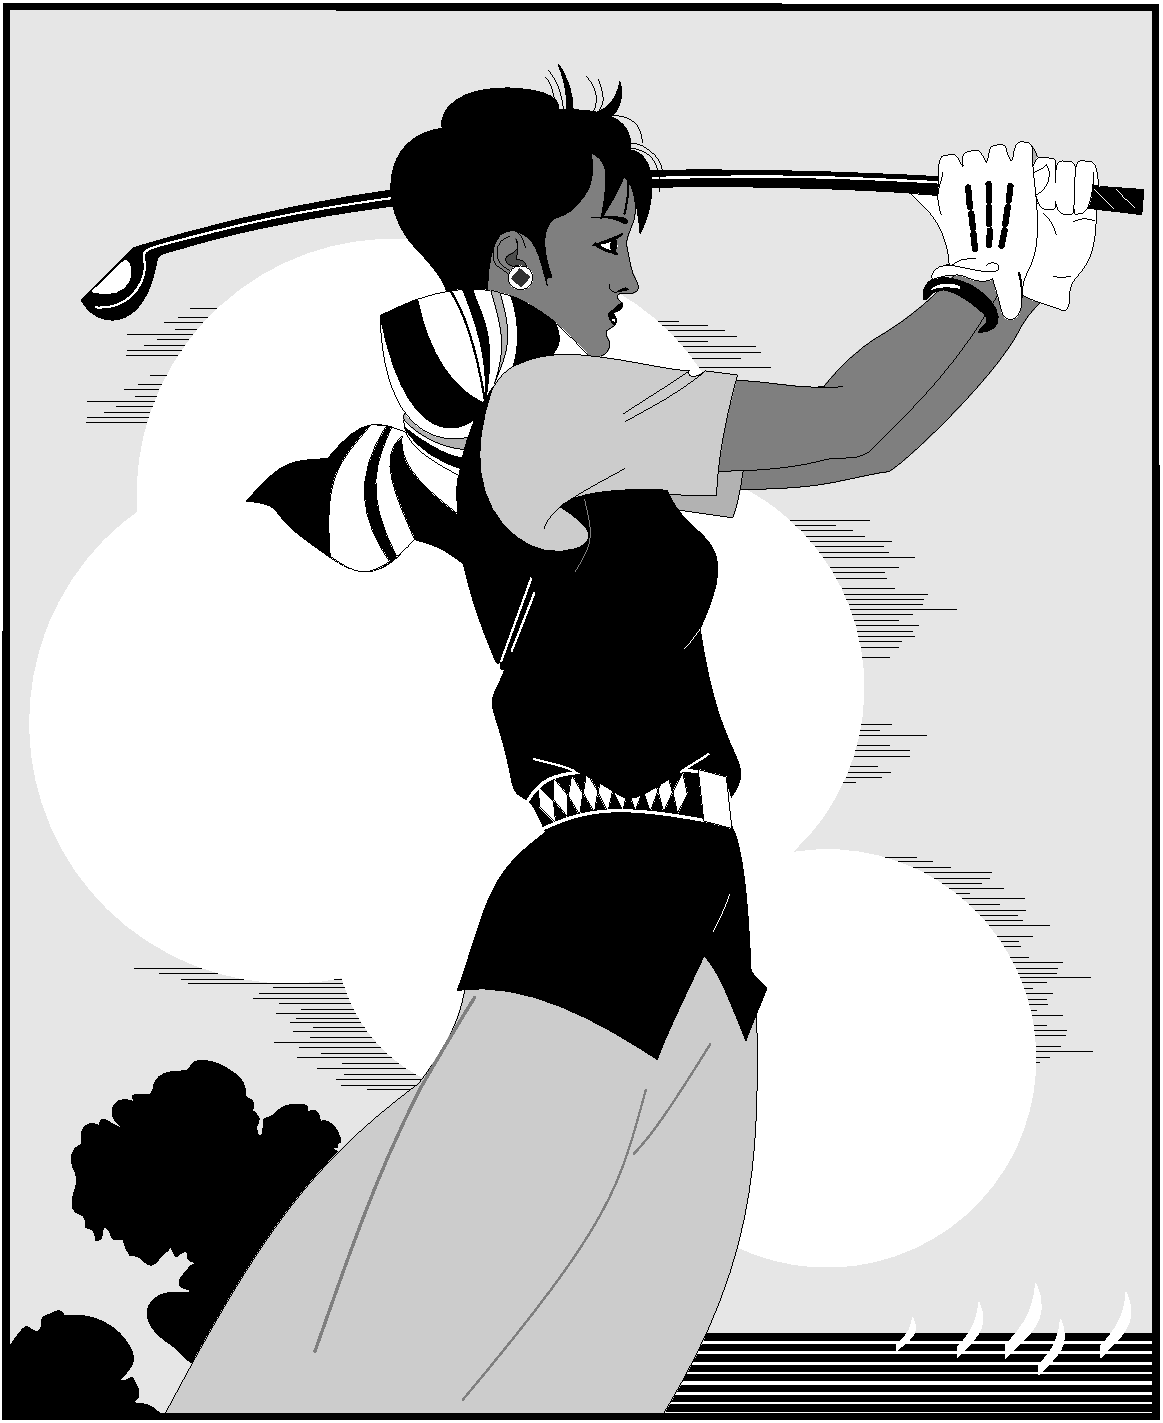
\includegraphics[width = 0.4\textwidth]{golfer}
\FigureBiCaption{打高尔夫球的人}{Golfer}
\label{Figure:Tricks:Example1}
\end{figure}

如果某图题很长的话,可以通过局部改变\verb|\captionwidth|的宽度进行断行。
图~\ref{Figure:Tricks:Example11}给出了一个中英文标题过长的例子。

\begin{figure}[htbp]
\centering
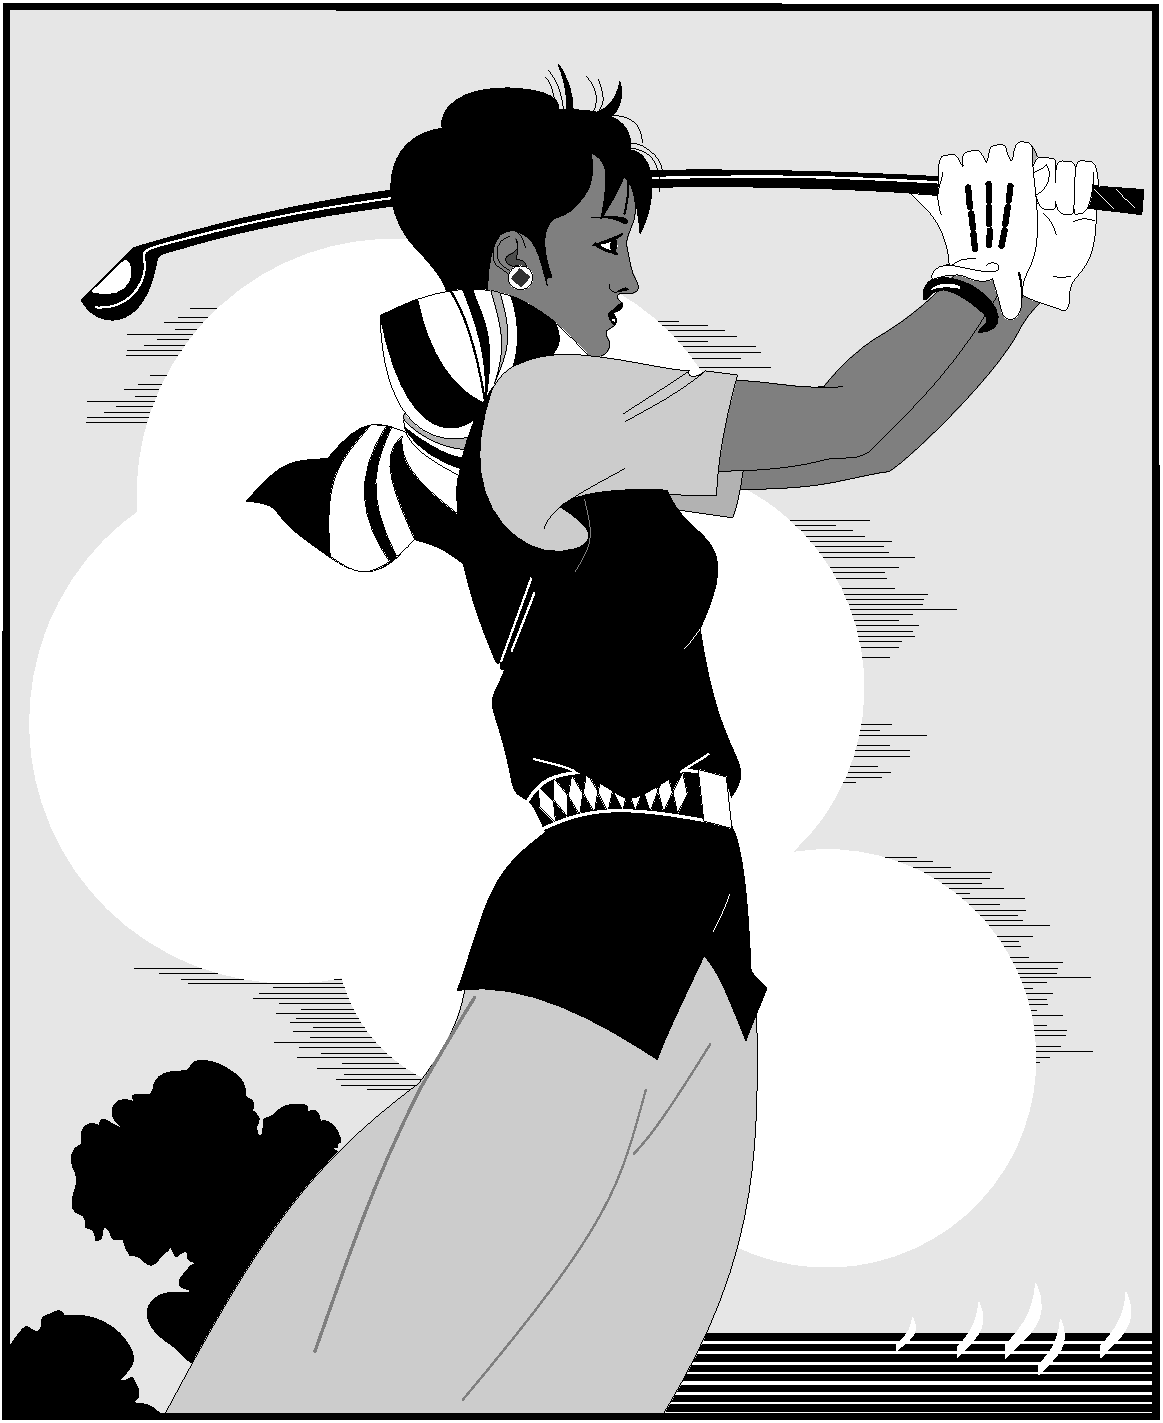
\includegraphics[width = 0.4\textwidth]{golfer}
\changecaptionwidth \captionwidth{0.7\textwidth}
\FigureBiCaption{一个打高尔夫球的人打 高尔夫球的人打高尔打
高尔夫球的人 打高尔 夫球的人打高尔夫球 的人打高尔夫球的
人打高尔夫球的人}{Golfer Golfer This is a very good idea and i
like it very much do u like it Golfer Golfer Golfer Golfer Golfer
Golfer Golfer Golfer Golfer} \label{Figure:Tricks:Example11}
\end{figure}

\normalcaptionwidth
图~\ref{Figure:Tricks:Example12}是恢复默认宽度之后的图形例子。
\begin{figure}[htbp]
\centering
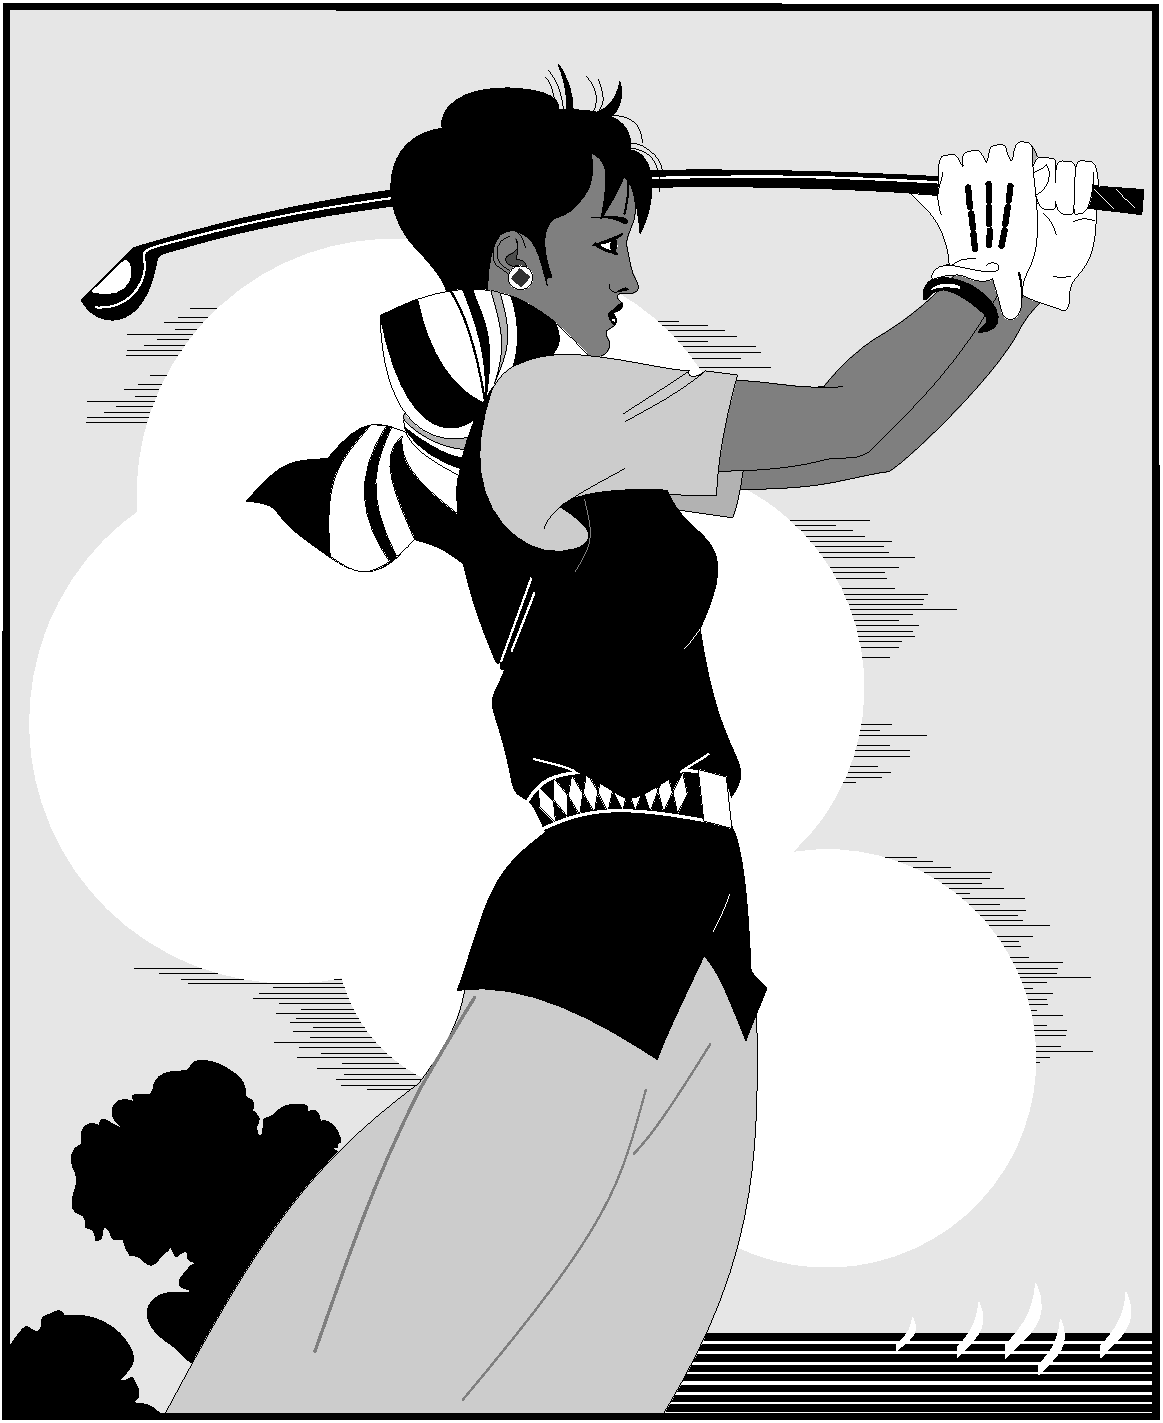
\includegraphics[width = 0.4\textwidth]{golfer}
\FigureBiCaption{打高尔夫球的人打高尔夫球的人打高尔打高尔夫球的人打高尔夫球的人打高尔夫球的人打高尔夫球的人打高尔夫球的人}{Golfer Golfer Golfer Golfer Golfer Golfer   Golfer Golfer Golfer Golfer Golfer Golfer Golfer Golfer Golfer Golfer Golfer Golfer}
\label{Figure:Tricks:Example12}
\end{figure}


为子图定义了一个英文标题命令:
\begin{verb}
\SubfigEnCaption{英文}。
\end{verb}
在紧接着~subfigure~后面用这个命令,参数是英文标题。
当一行不只一个子图时,将图放在~minipage~中,在~minipage~中用这个命令。

图~\ref{Figure:Tricks:Example2} 给出了一行只有一个子图的例子。

图~\ref{Figure:Tricks:Example3} 给出了一行有多个子图的例子。

\begin{figure}[htbp]
\centering
\begin{minipage}{0.40\textwidth}
\centering
\subfigure[高尔夫1]{\label{Figure:Tricks:Example2:a}
  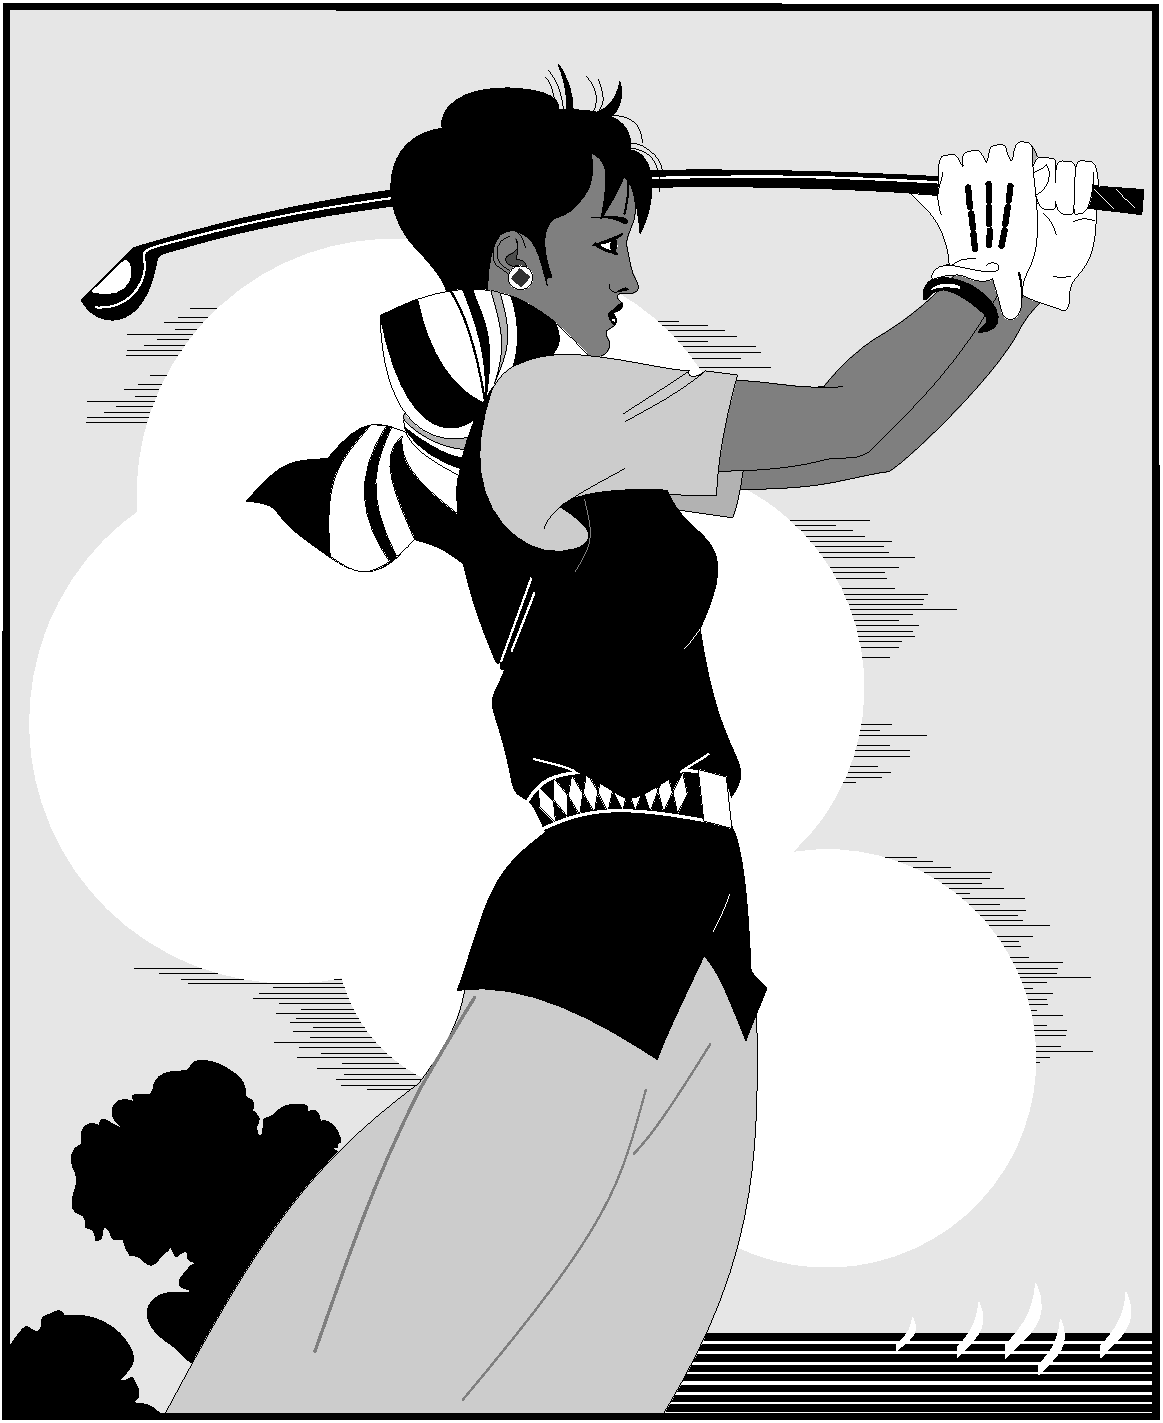
\includegraphics[width = \textwidth]{golfer}
}\SubfigEnCaption{Golfer1}
\end{minipage} 

\begin{minipage}{0.40\textwidth} %
\centering
\subfigure[高尔夫2]{\label{Figure:Tricks:Example2:B}
  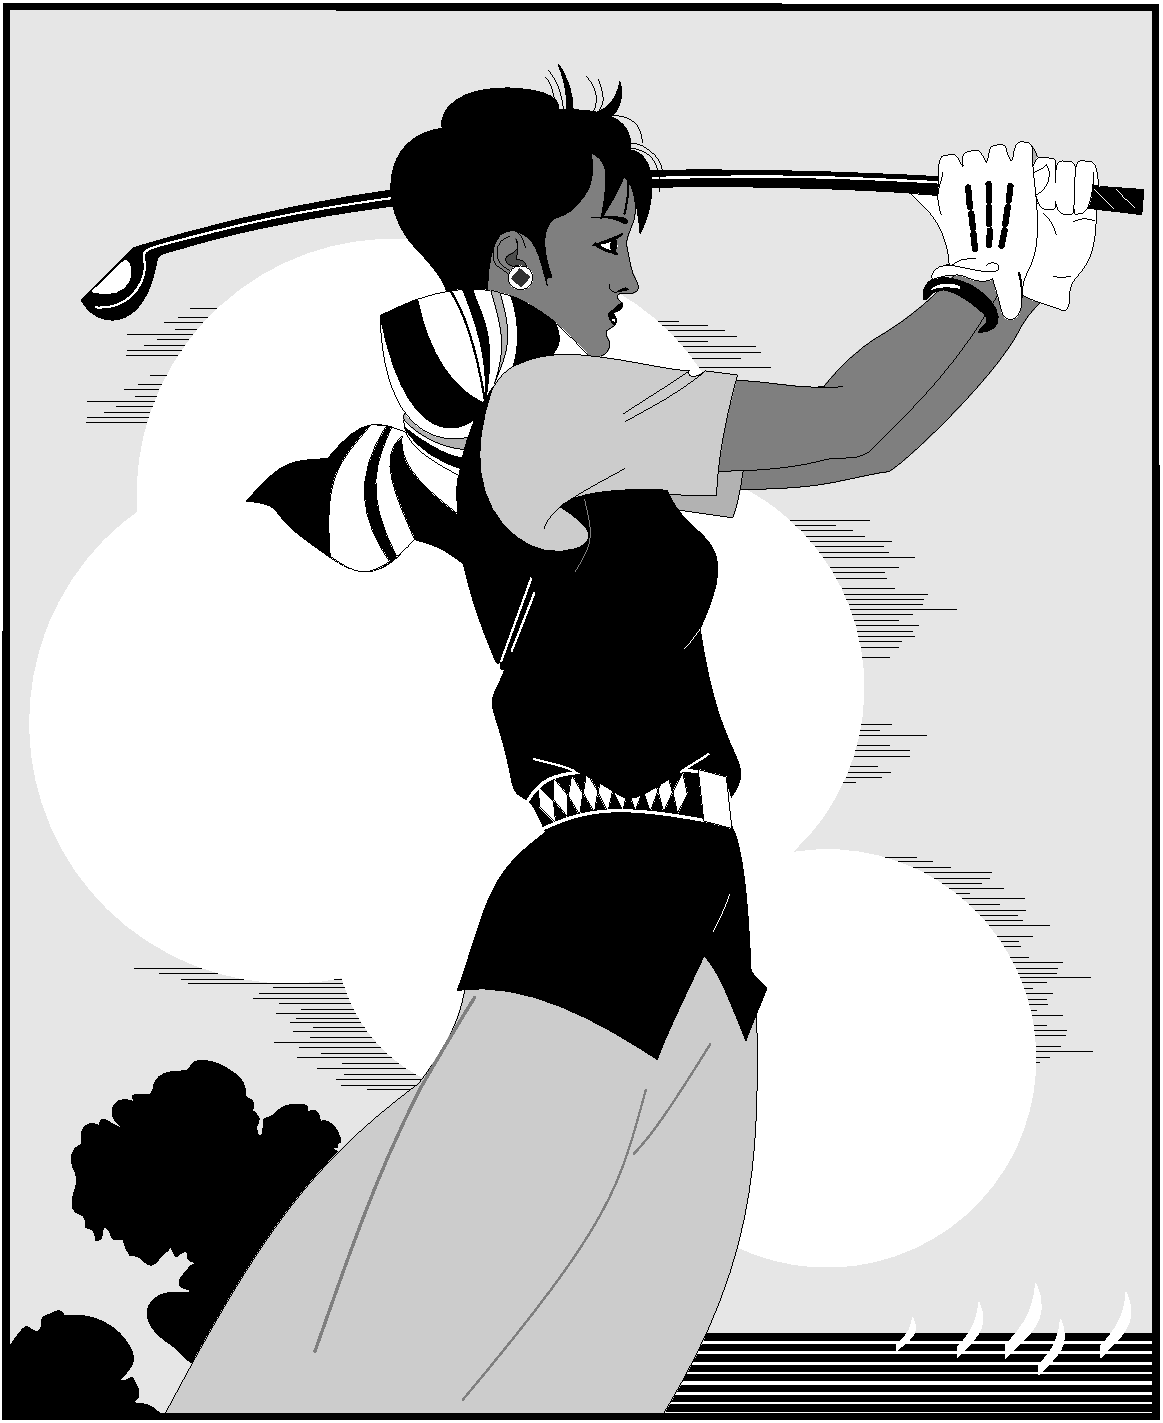
\includegraphics[width = \textwidth]{golfer}
}\SubfigEnCaption{$I_{\rm dc} = 0.5 III$A}
\end{minipage}
\FigureBiCaption{高尔夫}{Golf}
\label{Figure:Tricks:Example2222}
\end{figure}

\begin{figure}[htbp]
\centering
\begin{minipage}{0.25\textwidth}
\centering
\subfigure[高尔夫1]{\label{Figure:Tricks:Example3:a}
  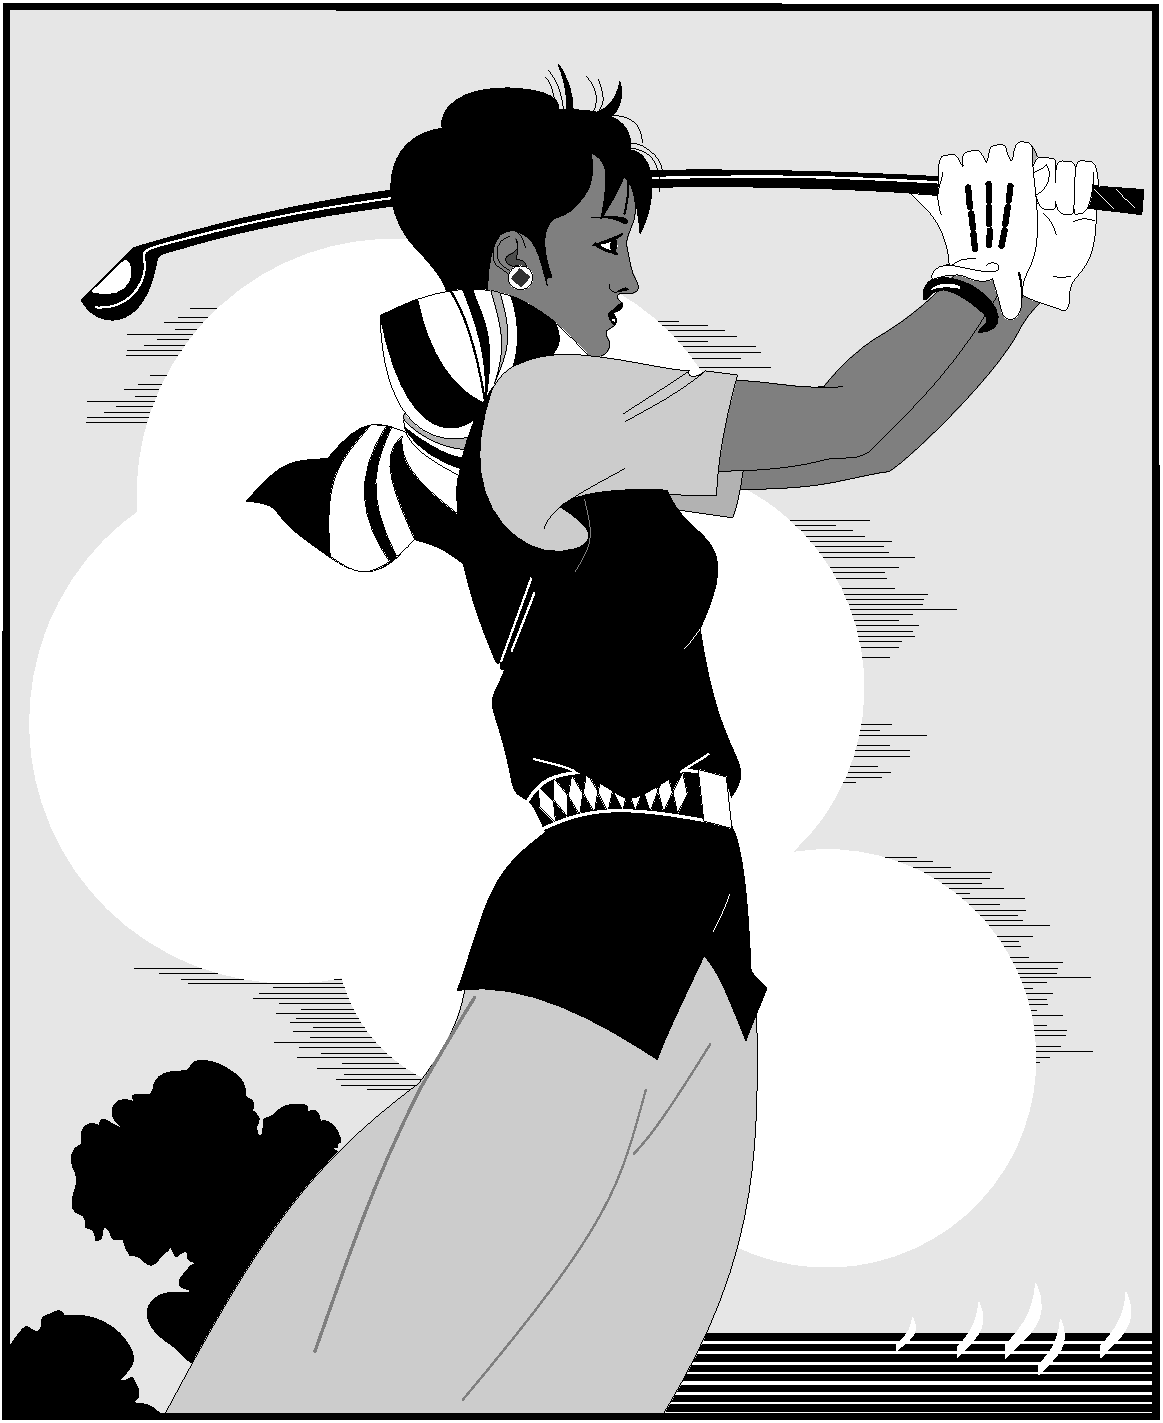
\includegraphics[width = \textwidth]{golfer}
}\vspace*{-5pt}\SubfigEnCaption{Golfer1}
\end{minipage}
\begin{minipage}{0.25\textwidth}
\centering
\subfigure[高尔夫2]{\label{Figure:Tricks:Example3:B}
  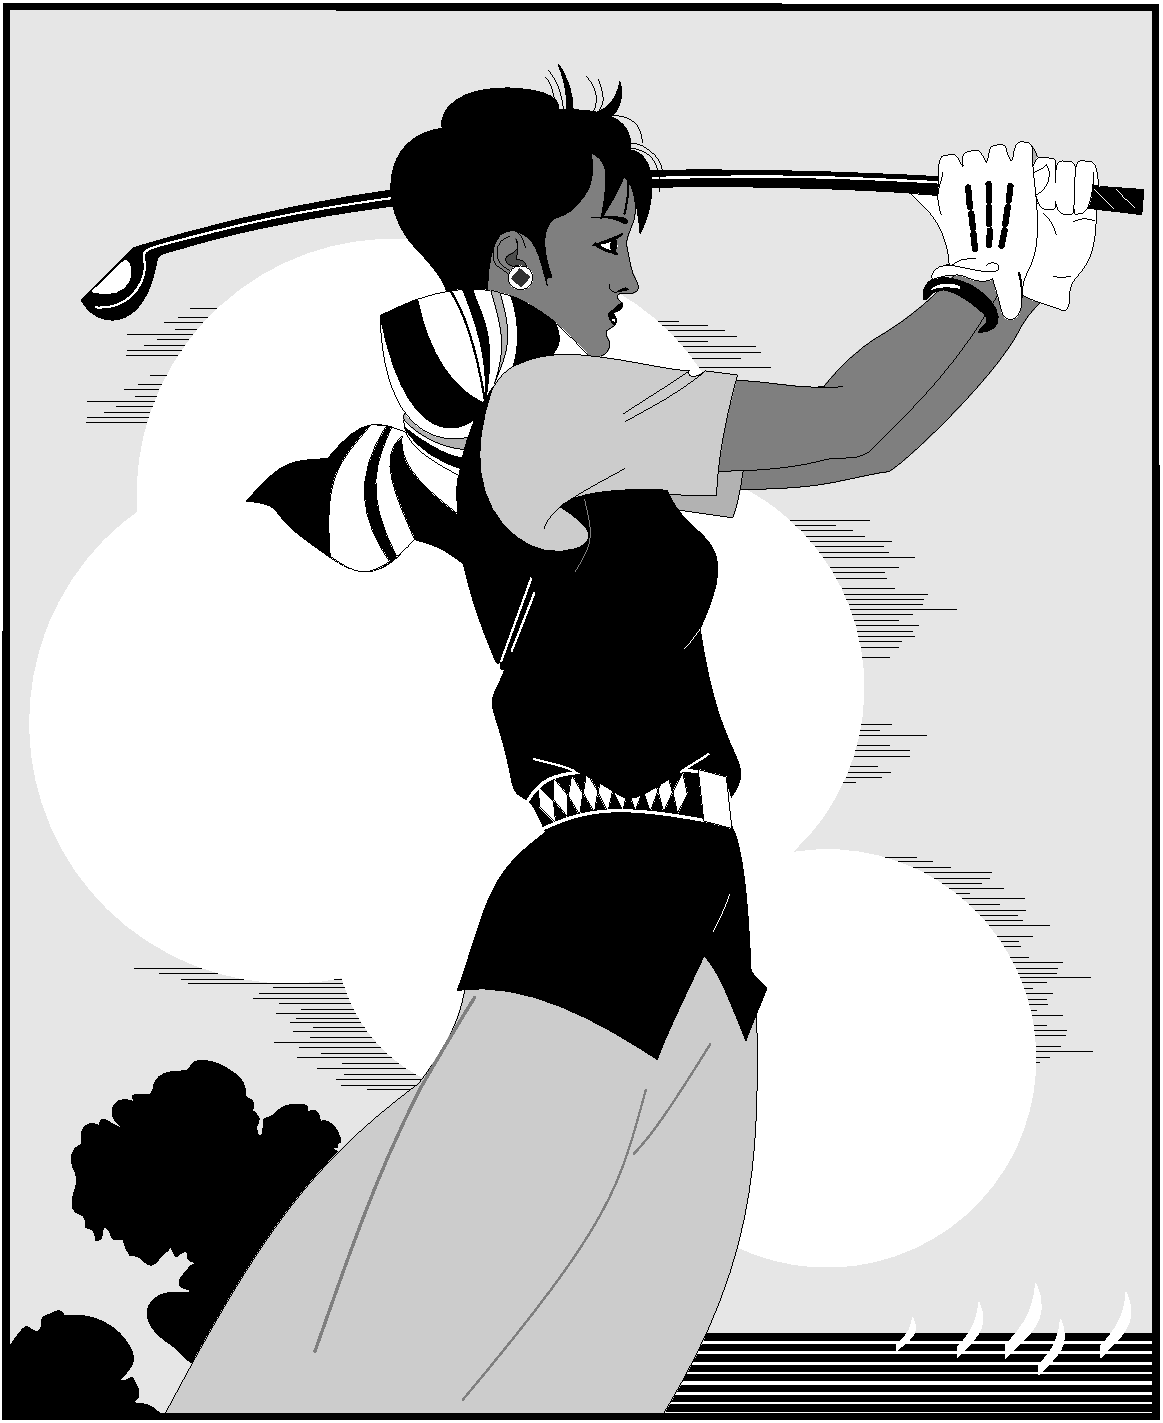
\includegraphics[width = \textwidth]{golfer}
}\vspace*{-5pt}\SubfigEnCaption{Golfer2}
\end{minipage}
\begin{minipage}{0.25\textwidth}
\centering
\subfigure[高尔夫3]{\label{Figure:Tricks:Example3:C}
  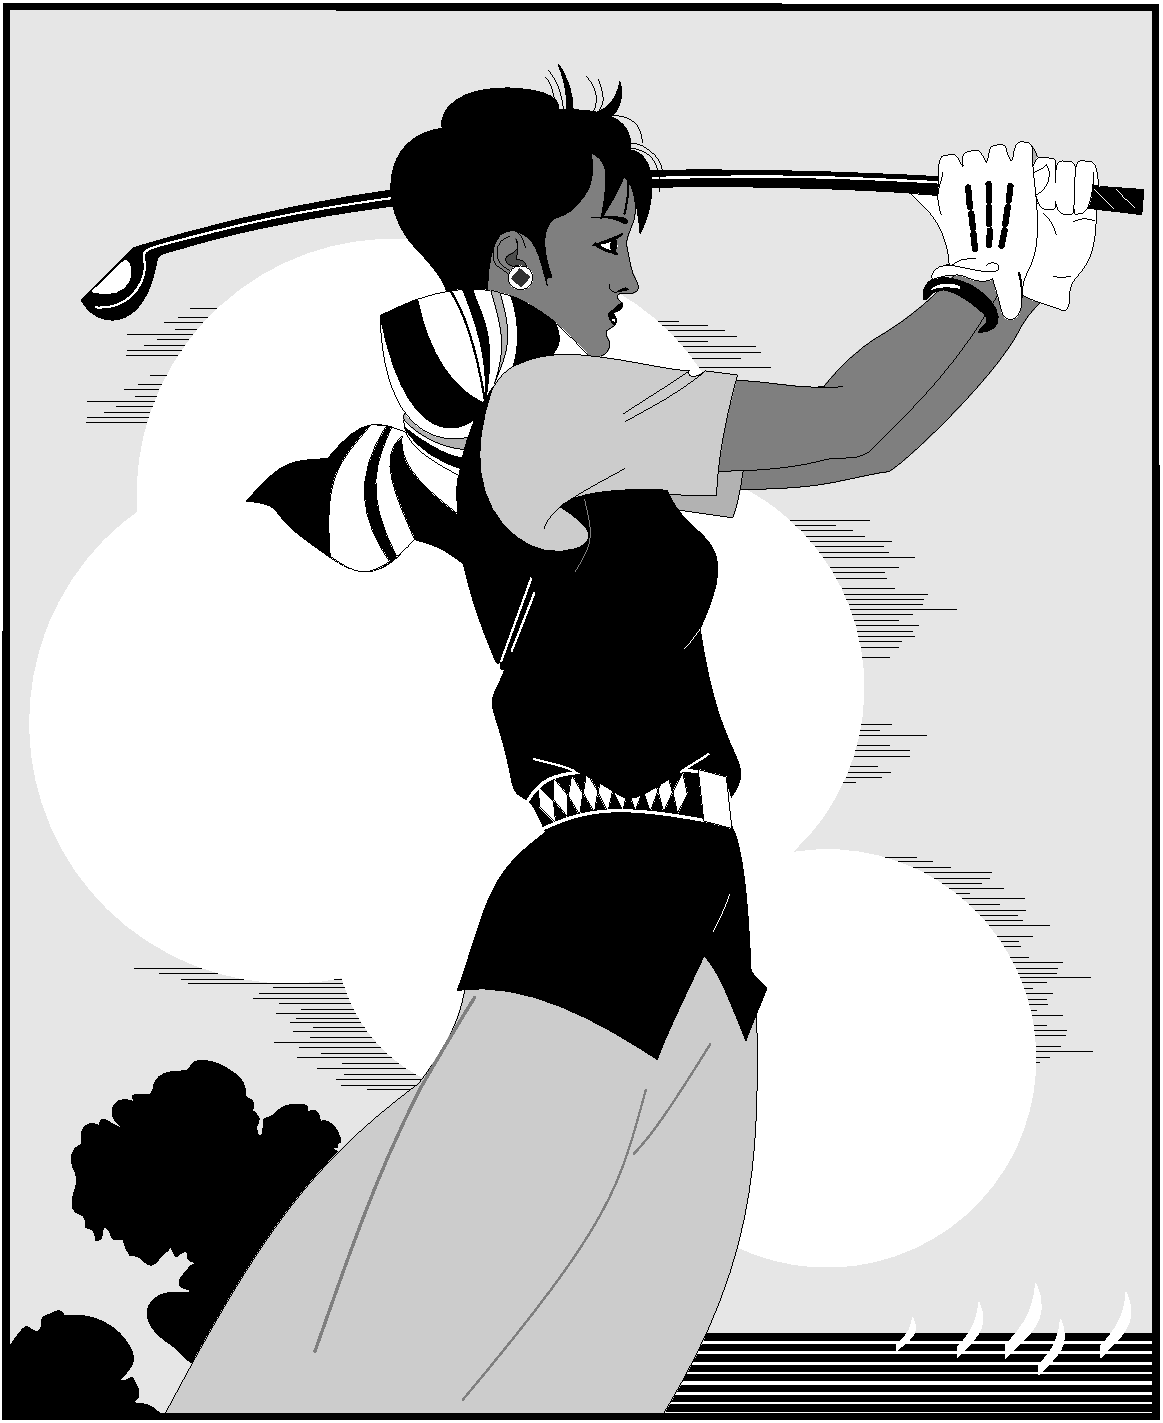
\includegraphics[width = \textwidth]{golfer}
}\vspace*{-5pt}\SubfigEnCaption{Golfer3}
\end{minipage}
\FigureBiCaption{高尔夫}{Golf}
\label{Figure:Tricks:Example3}
\end{figure}

图~\ref{Figure:Tricks:Example3x} 给出了一个不同大小子图的例子,这时可以给出分图的标号,然后把分图的图题
放到母图图题的下面。
\begin{figure}[htbp]
\centering
\begin{minipage}[b]{0.45\textwidth}
\centering
\subfigure[]{\label{Figure:Tricks:Example3x:a}
  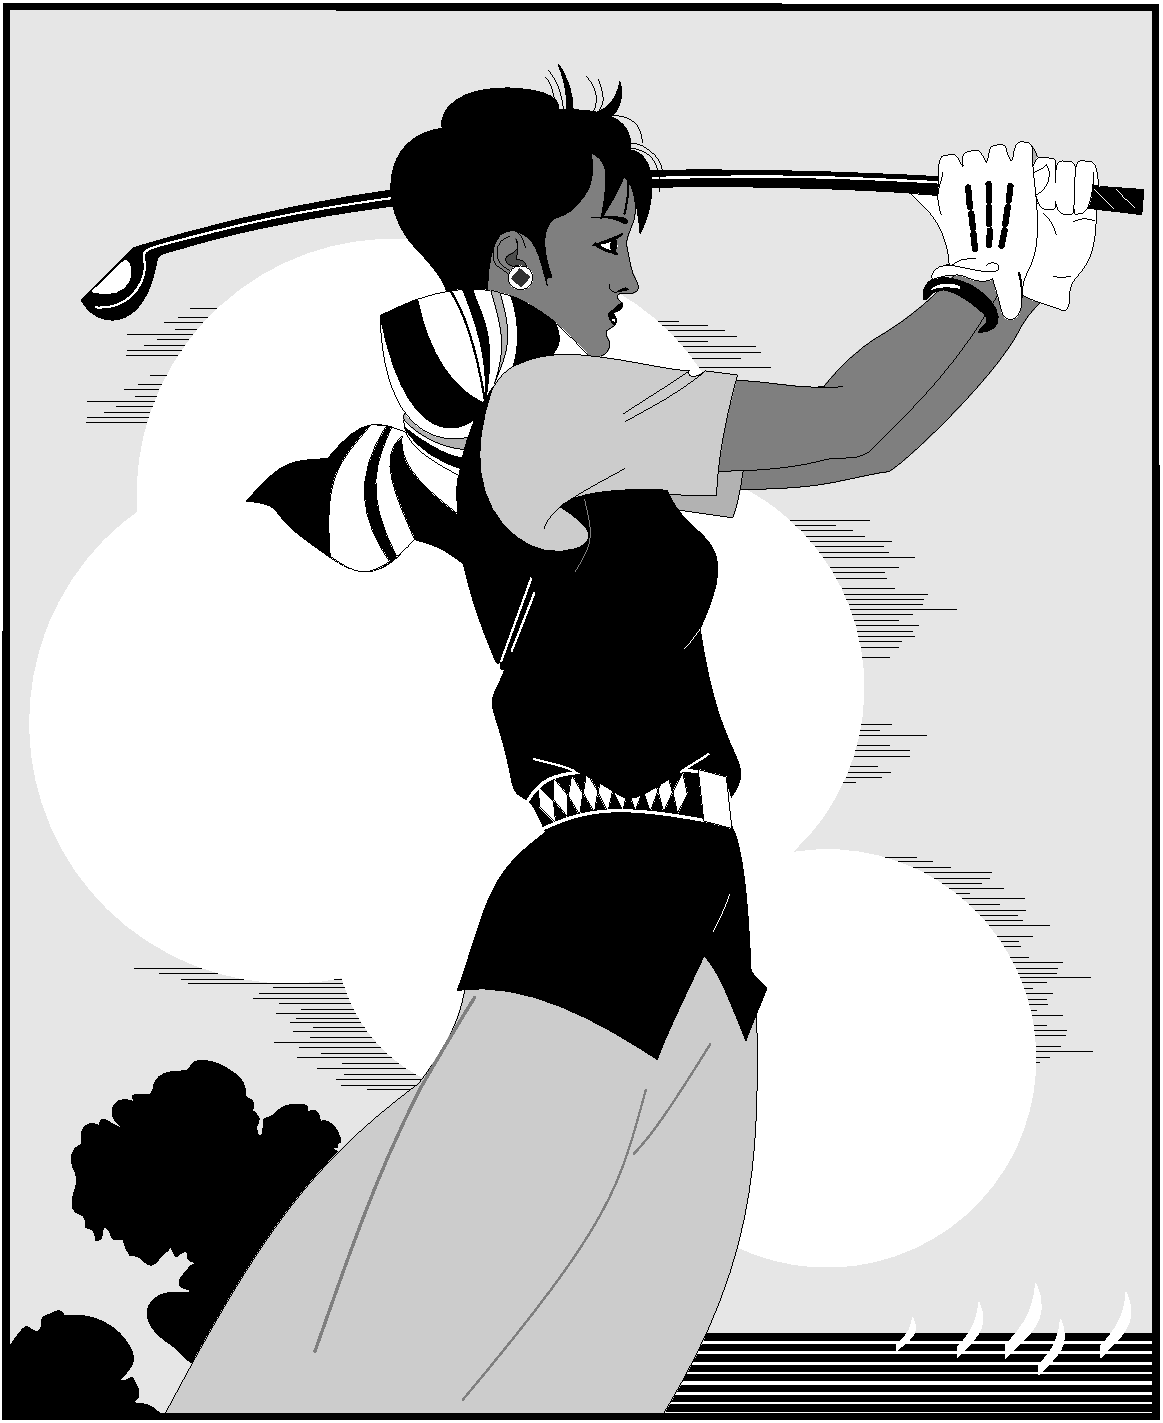
\includegraphics[width = \textwidth]{golfer}
}\vspace*{-5pt}
\end{minipage}
\begin{minipage}[b]{0.15\textwidth}
\centering
\subfigure[]{\label{Figure:Tricks:Example3x:B}
  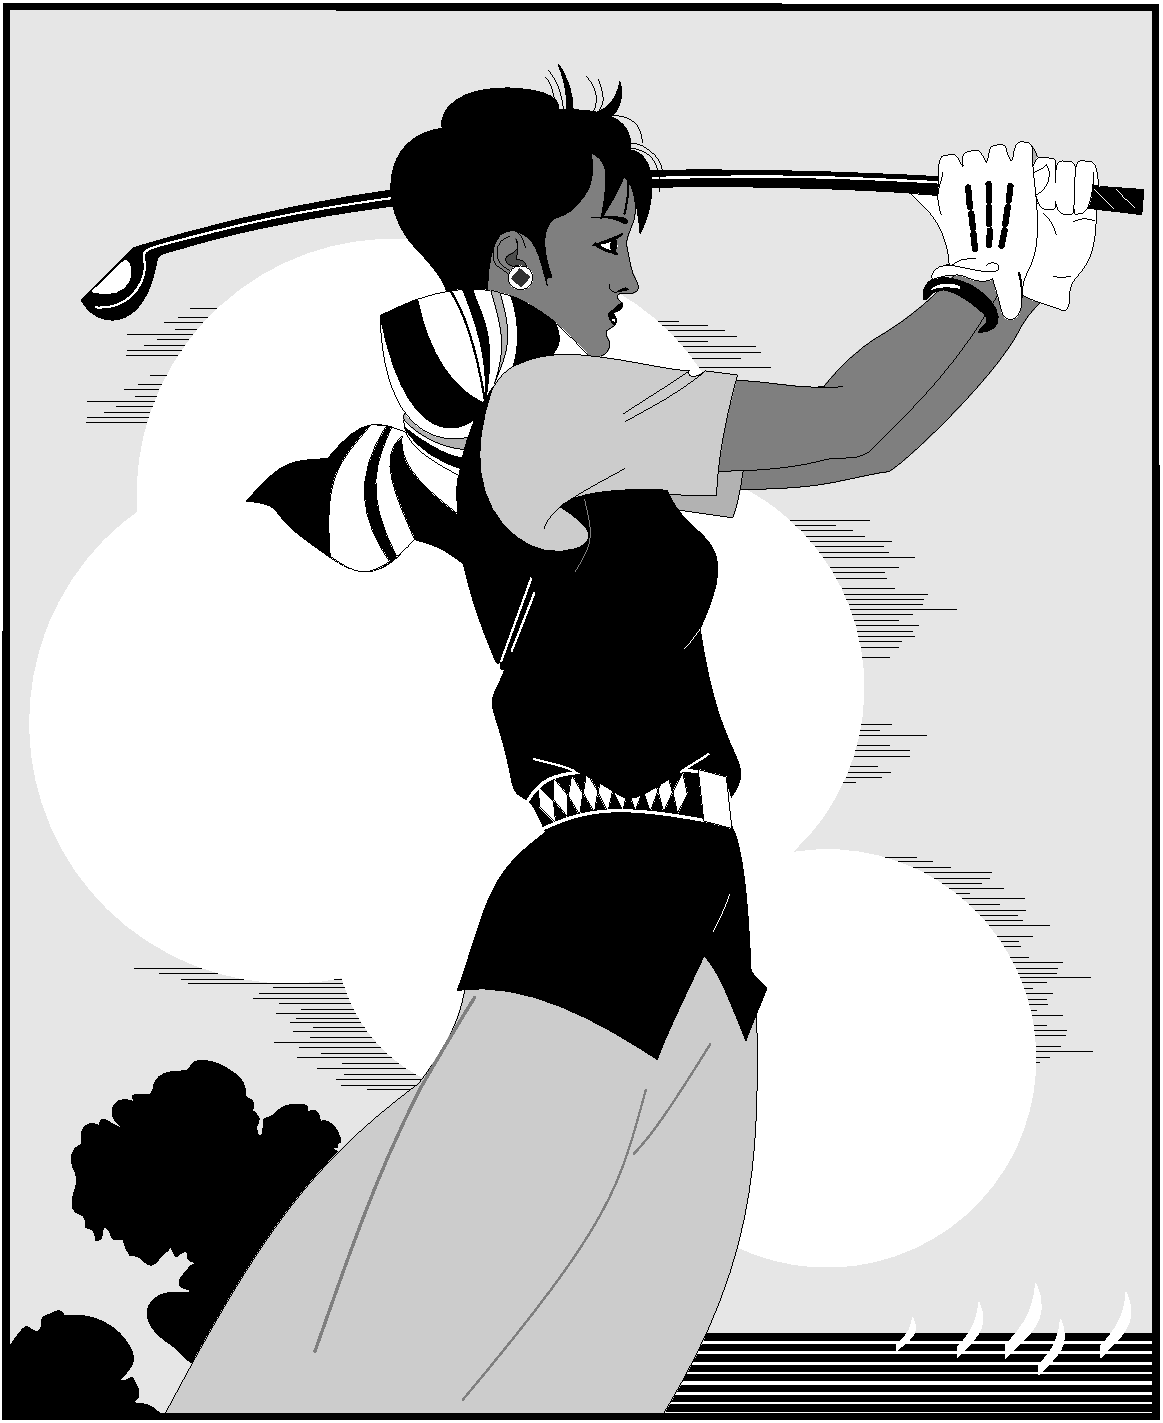
\includegraphics[width = \textwidth]{golfer}
}\vspace*{-5pt}
\end{minipage}
\begin{minipage}[b]{0.15\textwidth}
\centering
\subfigure[]{\label{Figure:Tricks:Example3x:C}
  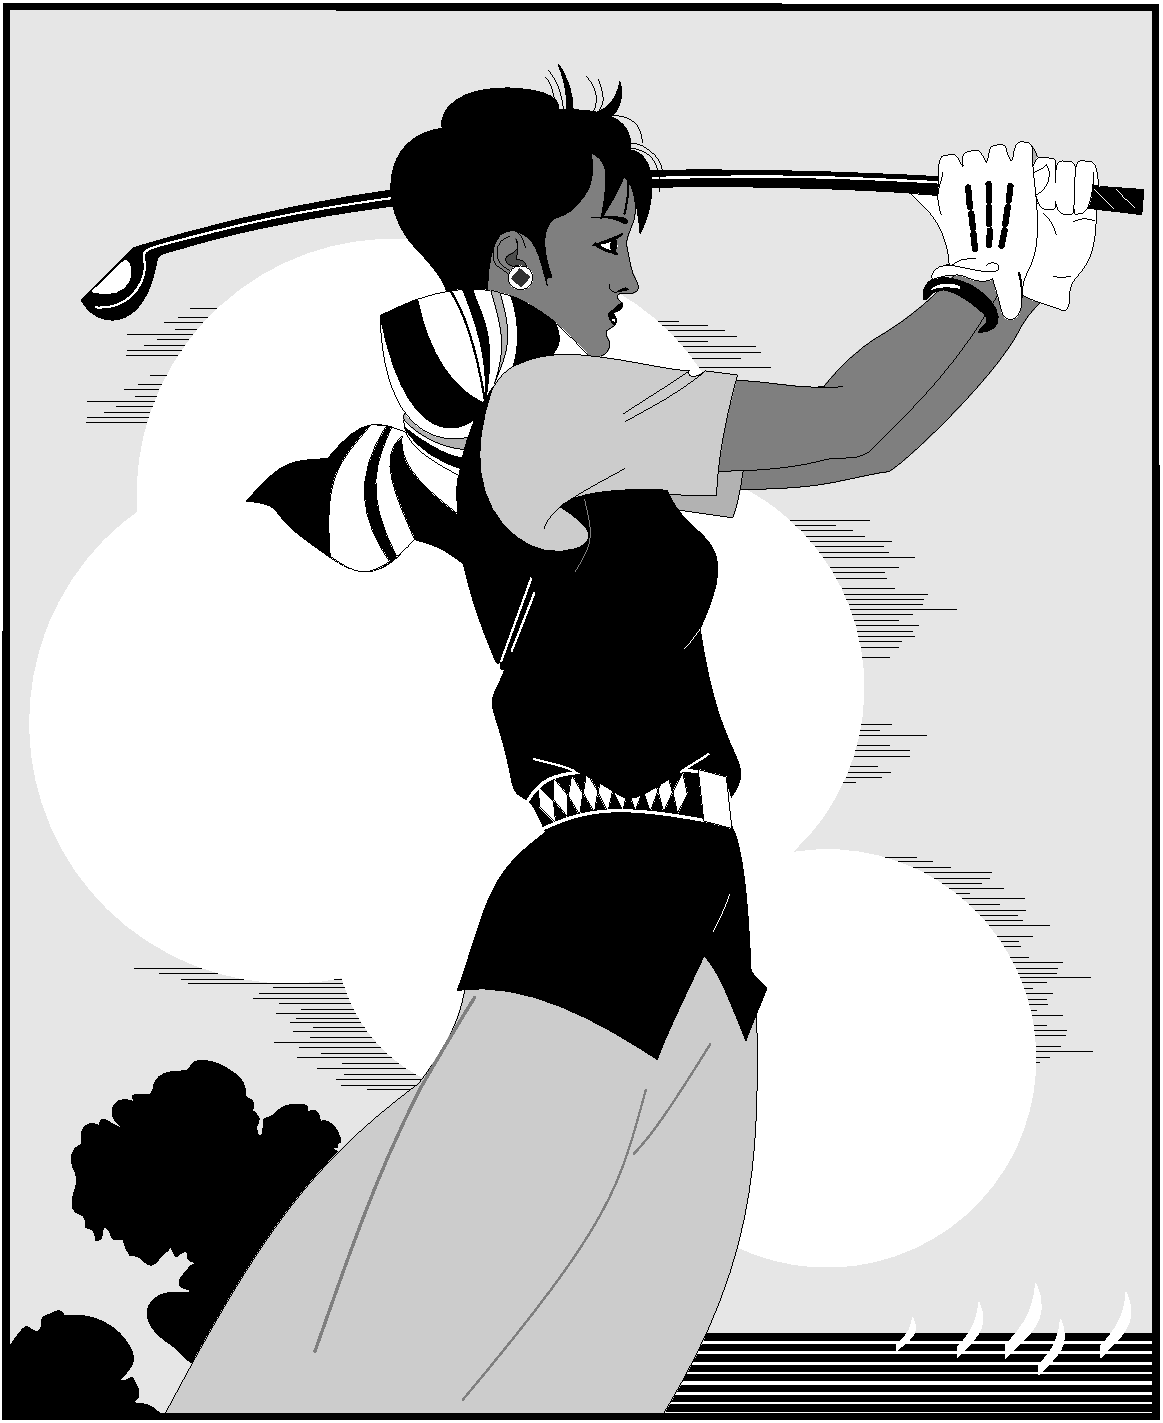
\includegraphics[width = \textwidth]{golfer}
}\vspace*{-5pt}
\end{minipage}
\FigureBiCaption{  高尔夫 \protect \\ a) 分图一; b) 分图二; c) 分图三}%
{  figure caption \protect \\ a) the first subfigure; b) the second subfigure; c) the third subfigure }
\label{Figure:Tricks:Example3x}
\end{figure}


图~\ref{Figure:Tricks:Example31} 给出了一个子图图题过长的例子
\begin{figure}[htbp]
\centering
\begin{minipage}[t]{0.20\textwidth}
\centering
\subfigure[高尔夫高尔夫高尔夫高尔夫1]{\label{Figure:Tricks:Example31:a}
  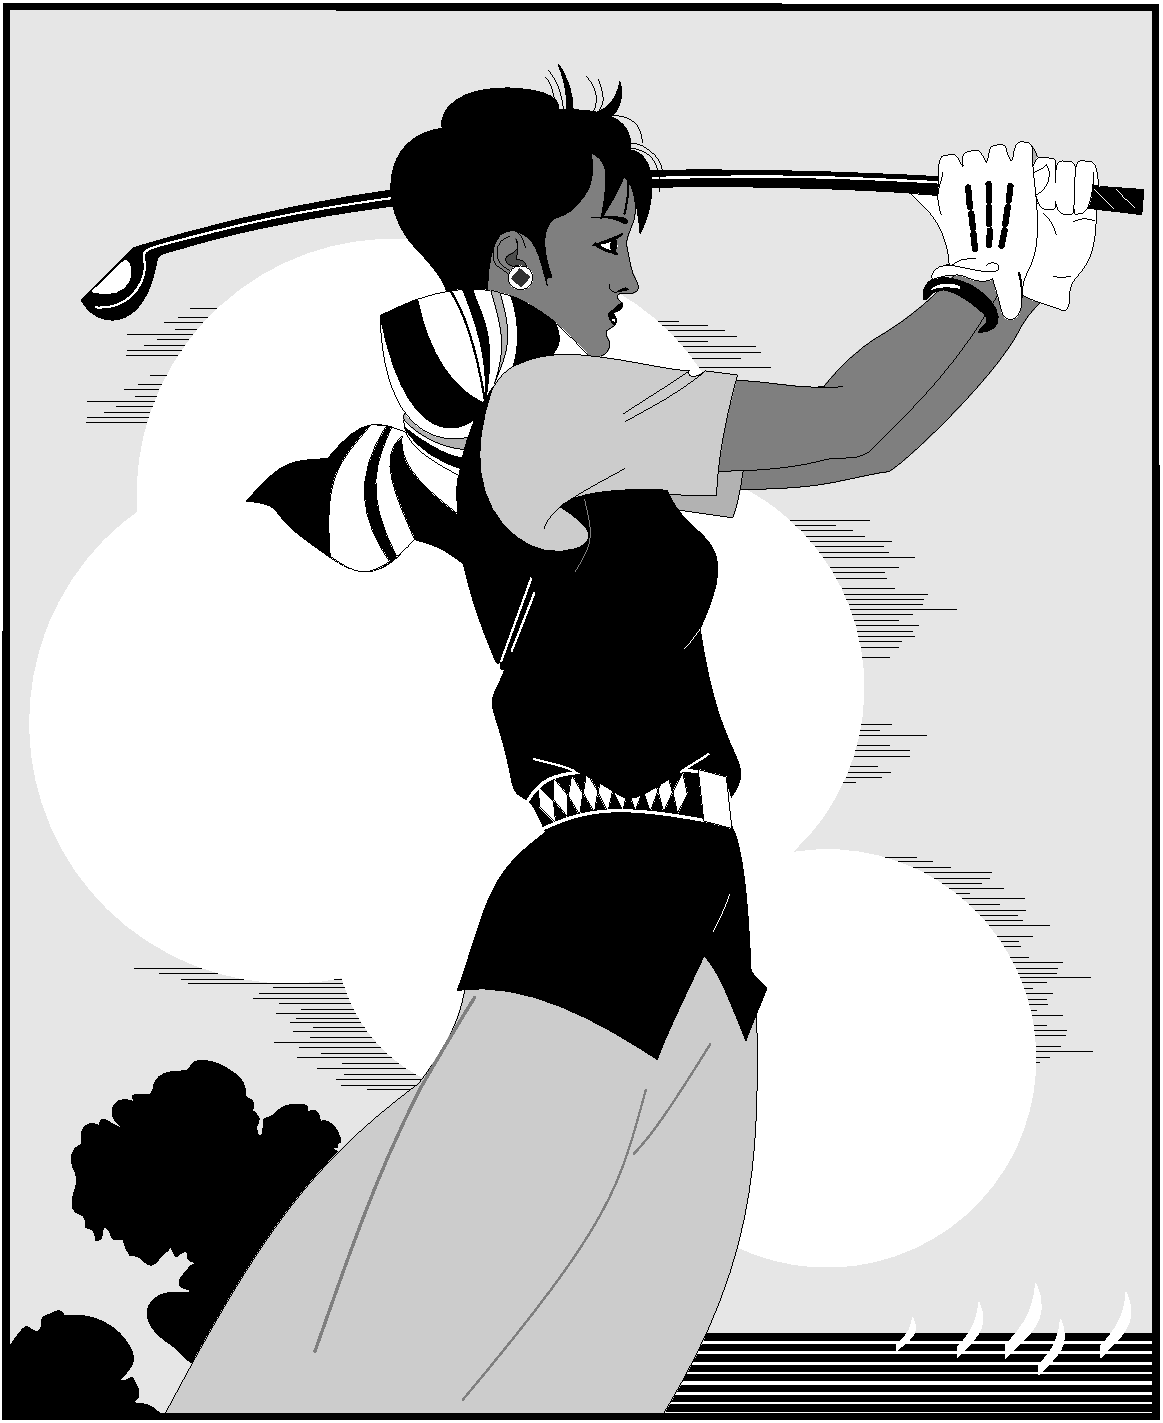
\includegraphics[width = \textwidth]{golfer}
}\SubfigEnCaption{Golfer1 Golfer1 Golfer1 Golfer1 Golfer1}
\end{minipage}\hspace{2em}
\begin{minipage}[t]{0.20\textwidth}
\centering
\subfigure[高尔夫高尔夫高尔夫高夫2]{\label{Figure:Tricks:Example31:B}
  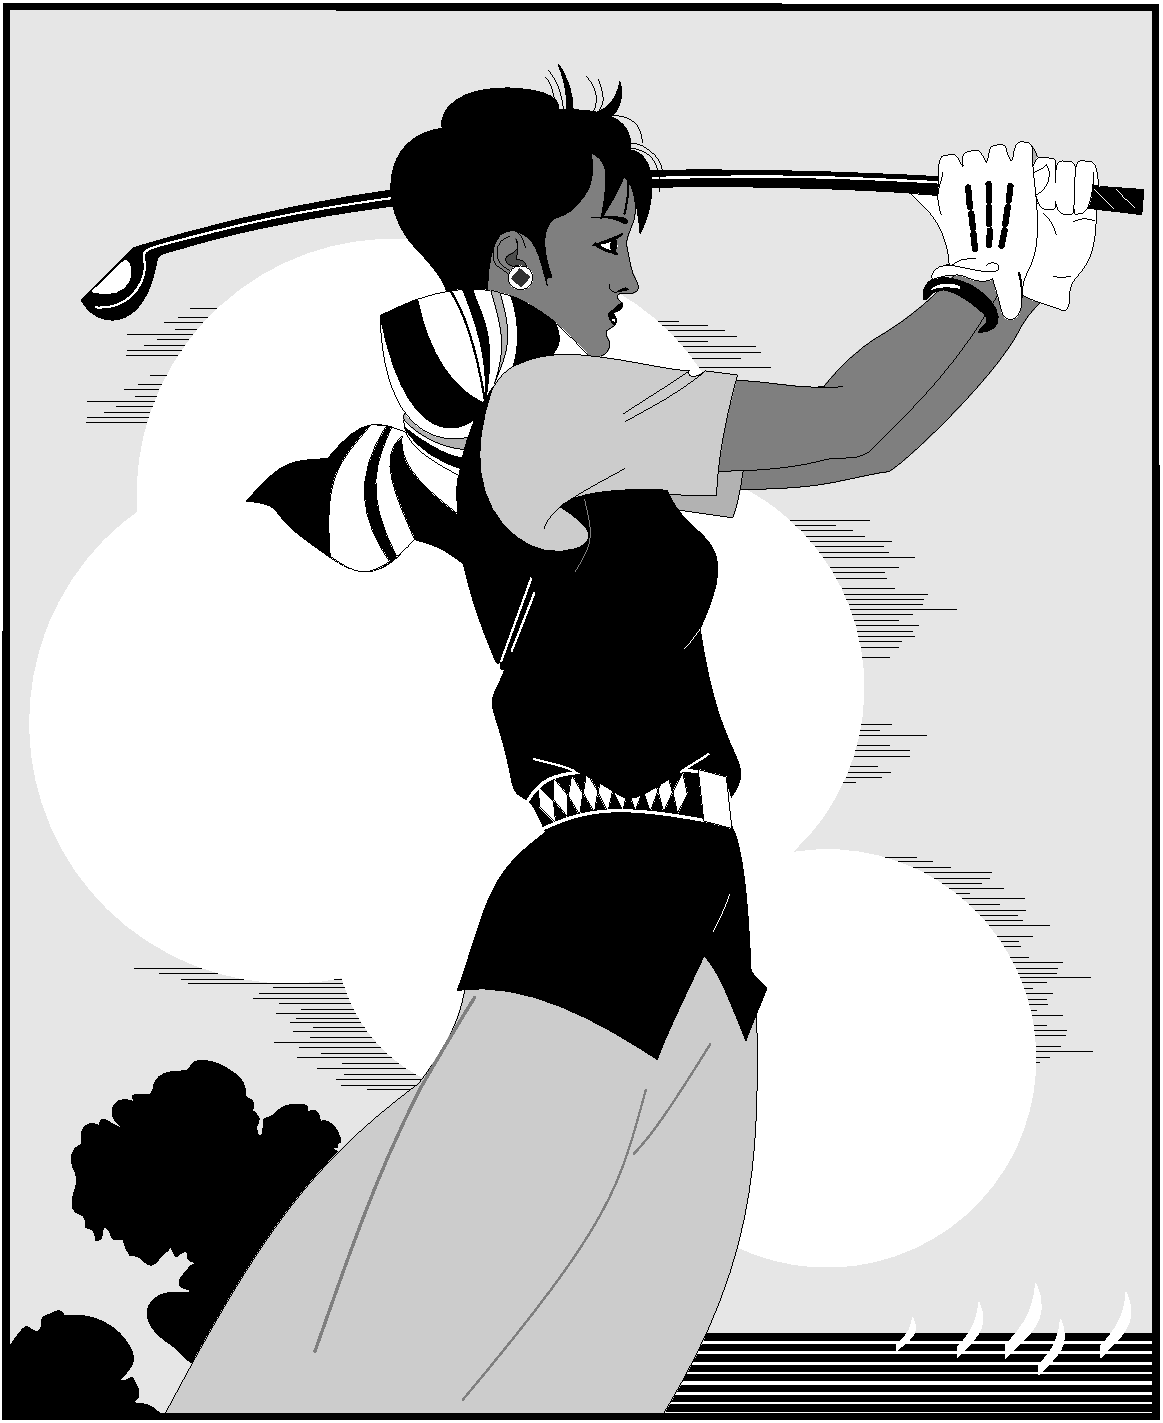
\includegraphics[width = \textwidth]{golfer}
}\SubfigEnCaption{G G f f f f f f f f f f f f f f f f f f}
\end{minipage}\hspace{2em}
\begin{minipage}[t]{0.20\textwidth}
\centering
\subfigure[高尔夫高尔夫高尔夫高尔3]{\label{Figure:Tricks:Example31:C}
  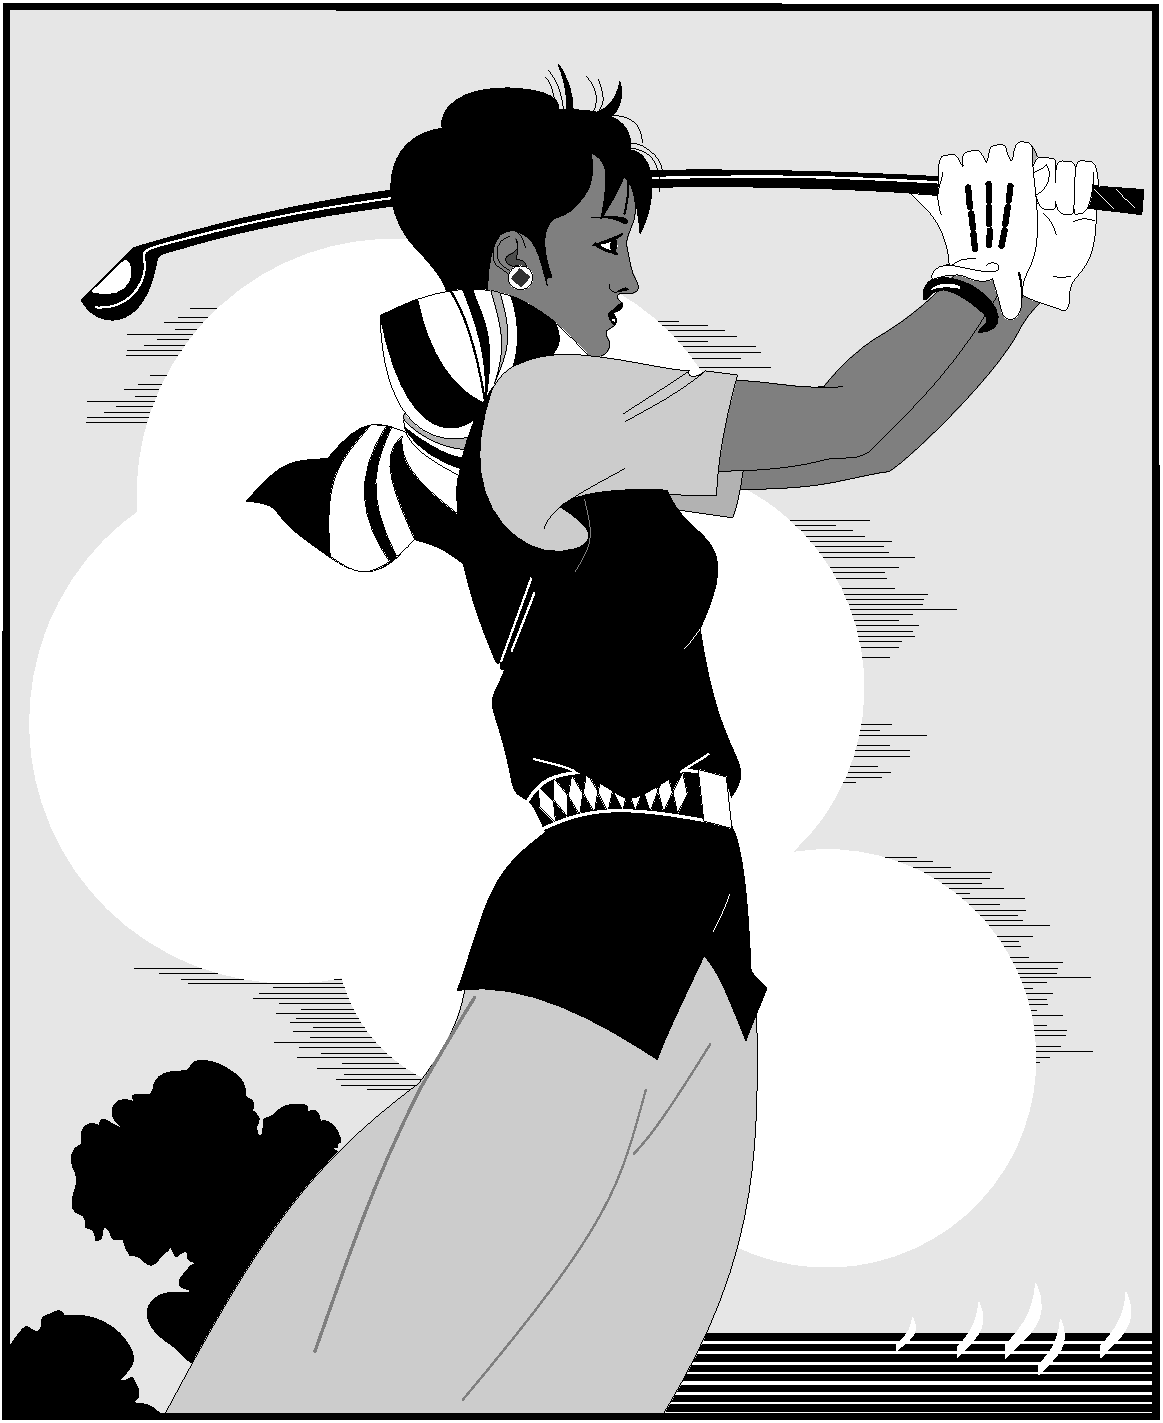
\includegraphics[width = \textwidth]{golfer}
}\SubfigEnCaption{Golfer3 Golfer3 Golfer3 Golfer3 Golfer3 Golfer3}
\end{minipage}
\FigureBiCaption{总图:高尔夫 高尔夫 高尔夫 高尔夫 高尔夫}{Parent: Golf Golf Golf Golf Golf}
\label{Figure:Tricks:Example31}
\end{figure}


\BiSubsection{表标题}{Caption of Tables}
模板中分别为表定义了双标题命令:
\verb"\TableBiCaption{中文}{英文}"。
该命令含有两个参数,第一个为中文标题,第二个为英文标题,效果见~\ref{Tricks:Tab1}。


\begin{table}[htbp]
\centering 
\TableBiCaption{表格测试}{Test of Table}
\label{Tricks:Tab1}
\begin{tabular}{c|c|c}
  \hline
  % after \\: \hline or \cline{col1-col2} \cline{col3-col4} ...
  方法 & 精度~(\%) & 速度~(ms) \\
  \hline
  小波变换 & $99.8$ &  20\\
  傅立叶变换 & $99.0$ & 30 \\
  \hline
\end{tabular}
\end{table}

对于长表格的中英文标题,采用~\verb"\LTBiTocCaption{中文长表短标题(目录中)}{中文长表长标题(正文中)}{Table}{英文长表短标题(目录中)}{英文长表长标题(正文)}"
~来定义。需要注意的是,该命令借鉴了~\verb|ccaption| 宏包中的长表格标题处理方式,含有5个参数,
第三个参数无需改变,由于其他命令限制,参数不容易减少,所以如此定义。
采用这个命令,长表格的标题在正文和图表目录均能正常排版,并且和其他表格的编号协调。
如果需要引用长表格,在~\verb|\LTBiTocCaption|命令之后紧接~\verb|\label| 命令。
表~\ref{table:LTexample} 给出一个例子。

\begin{longtable}{lll} 
\LTBiTocCaption{中文标题短}{中文标题长}{Table}{Long Table  Short Caption}{Long Table Long Caption}\label{table:LTexample}\\
\bfseries Entity & \bfseries Unicode Name & \bfseries Unicode \\ \hline
\endfirsthead
\bfseries Entity & \bfseries Unicode Name & \bfseries Unicode \\ \hline
\endhead
\hline \multicolumn{3}{r}{\emph{Continued on next page}}
\endfoot
\hline
\endlastfoot
a&bcd&bcdef\\
表格&中文文字&中文\\
a&emf&bcdef\\
a&emf&bcdef\\
a&emf&bcdef\\
a&emf&bcdef\\
a&emf&bcdef\\
a&emf&bcdef\\
a&emf&bcdef\\
a&emf&bcdef\\
a&emf&bcdef\\
a&emf&bcdef\\
a&emf&bcdef\\
a&emf&bcdef\\
a&emf&bcdef\\
a&emf&bcdef\\
a&emf&bcdef\\
a&emf&bcdef\\
a&emf&bcdef\\
a&emf&bcdef\\
%a&emf&bcdef\\
\end{longtable}



\BiSection{算法}{algorithm}
这是一个算法的例子,来自~worldguy@lilacbbs~
\begin{algorithm}
\KwIn{training samples, {$(d_i, d_j)_q$; $\mathbf{q}_i, \mathbf{q}_j \in C$,
$q\in \mathbf{Q}$} }
\KwOut{parameter setting $\lambda^T$}

\For{$t$=1 to $T$}
{   
    $\lambda^{t+1}_n = \lambda^t_n + \eta (f_n(q, c, d_i) - f_n(q, c, d_j))$
 }
\end{algorithm}
算法环境中右侧空白比较多,若想把右侧的空白框减小,可以采用minipage环境实现。把algorithm环境放到minipage环境里面,并且加上选项[H]禁止算法浮动,下面给出一个例子。需要说明的是,一般不需要进行这种处理。算法图题可有可无,若有中英文图题,请使用\verb|\AlgoBiCaption{中文图题}{英文图题}|。下面给出两个有图题的例子。需要说明的是,算法和图表的图题一样,都是自动换行,没有必要手动换行,如果采用\verb|\protect\\|手动换行,会造成目录中也是同样的手动换行,不符合常规排版要求。

\begin{minipage}{0.8\textwidth}\centering
\begin{algorithm}[H]
 \AlgoBiCaption{这是一个简短的算法中文图题}{This is the English caption of the algorithm}
  \KwIn{training samples, {$(d_i, d_j)_q$; $\mathbf{q}_i, \mathbf{q}_j
      \in C$, $q\in \mathbf{Q}$} }
 \KwOut{parameter setting
    $\lambda^T$}
 \For{$t$=1 to $T$} { $\lambda^{t+1}_n = \lambda^t_n +
    \eta (f_n(q, c, d_i) - f_n(q, c, d_j))$ }
\end{algorithm}
\end{minipage}


\begin{minipage}{0.9\textwidth}\centering
\begin{algorithm}[H]
 \AlgoBiCaption{这是一个算法的比较长的中文图题,需要换行,这里采用自动换行,如果手动换行会造成算法目录中同样出现断行}{This is a long English caption of the algorithm, a new line  required, and this a new line}
  \KwIn{training samples, {$(d_i, d_j)_q$; $\mathbf{q}_i, \mathbf{q}_j
      \in C$, $q\in \mathbf{Q}$} }
 \KwOut{parameter setting
    $\lambda^T$}
 \For{$t$=1 to $T$} { $\lambda^{t+1}_n = \lambda^t_n +
    \eta (f_n(q, c, d_i) - f_n(q, c, d_j))$ }
\end{algorithm}
\end{minipage}

\BiSection{公式}{Equations}
\label{Tricks:Equations}

文本中的数学符号和公式用下面的方法输入:

天体力学问题所采取的一个最基本的模型就是通常所说的$N$体问题,即在一
定条件下,所研究的天体被看成质点,$N$体问题最简单的就是二体问题。在一
个天体系统中,$N$个天体往往包含$n$个大天体和$k$个小天体($N=n+k$),其中
$k$个小天体相对$n$个大天体而言小到对后者运动的影响几乎不用考虑,但$k$
个小天体之间可能相距较近,它们之间的相互作用应予考虑,这就构成了限制
性($n+k$)体问题。特别地,当$N=3,~n=2,~k=1$时,即通常所说的限制性三体问题。


最基本的数学公式,带序号的:
\begin{equation}
\ddot{\mathbf{r}}=\mathbf{F}_{0}(r)+\mathbf{F}_{\varepsilon}(\mathbf{r},\dot{\mathbf{r}},t)
\end{equation}
\eqref{eq:noindex}是一个不带序号的例子:
\begin{displaymath}\label{eq:noindex}
F_{\varepsilon}/F_{0}=O (\varepsilon)
\end{displaymath}

\FloatBarrier %清除浮动体
典型的公式加符号说明的例子:

式\eqref{eq:1}为目标飞行器和追踪飞行器之间的相对运动方程
\begin{equation}\label{eq:1}
\ddot{\boldsymbol{\rho}}-\frac{\mu}{R_{t}^{3}}\left( 3\mathbf{R_{t}}\frac{\mathbf{R_{t}\rho}}{R_{t}^{2}}-\boldsymbol{\rho}\right)=\mathbf{a}
\end{equation}
其中:

$\boldsymbol{\rho}$---追踪飞行器与目标飞行器之间的相对位置矢量;

$\ddot{\boldsymbol{\rho}}$---追踪飞行器与目标飞行器之间的相对加速度;

$\mathbf{a}$---推力所产生的加速度;

$\mathbf{R}_{t}$---目标飞行器在惯性坐标系中的位置矢量;

$\omega_{t}$---目标飞行器的轨道角速度;

$\mathbf{g}$---重力加速度,$=\frac{\mu}{R_{t}^{3}}\left(
3\mathbf{R_{t}}\frac{\mathbf{R_{t}\rho}}{R_{t}^{2}}-\boldsymbol{\rho}\right)=\omega_{t}^{2}\frac{R_{t}}{p}\left(
3\mathbf{R_{t}}\frac{\mathbf{R_{t}\rho}}{R_{t}^{2}}-\boldsymbol{\rho}\right)$,这里$p$是目标飞行器的轨道半通径;

公式加符号说明还可以这样:
\begin{equation}\label{eq:111}
\ddot{\boldsymbol{\rho}}-\frac{\mu}{R_{t}^{3}}\left( 3\mathbf{R_{t}}\frac{\mathbf{R_{t}\rho}}{R_{t}^{2}}-\boldsymbol{\rho}\right)=\mathbf{a}
\end{equation}
\begin{formulasymb}{式中}{-15pt}%-3pt,-20pt调与上方的间距。
  \fdesfirst{$\boldsymbol{\rho}$}{追踪飞行器与目标飞行器之间的相对位置矢量;}
  \fdes{$\ddot{\boldsymbol{\rho}}$}{追踪飞行器与目标飞行器之间的相对加速度;}
  \fdes{$\mathbf{a}$}{推力所产生的加速度;}
  \fdes{$\mathbf{R}_{t}$}{目标飞行器在惯性坐标系中的位置矢量;}
  \fdes{$\omega_{t}$}{目标飞行器的轨道角速度;}
  \fdes{$\mathbf{g}$}{重力加速度,$=\frac{\mu}{R_{t}^{3}}\left(
3\mathbf{R_{t}}\frac{\mathbf{R_{t}\rho}}{R_{t}^{2}}-\boldsymbol{\rho}\right)=\omega_{t}^{2}\frac{R_{t}}{p}\left(
3\mathbf{R_{t}}\frac{\mathbf{R_{t}\rho}}{R_{t}^{2}}-\boldsymbol{\rho}\right)$,这里$p$是目标飞行器的轨道半通径;}
\end{formulasymb}

含有矩阵或者向量的公式:
\begin{equation}\label{eq:rho}
\dot{\boldsymbol{\rho}}=\left( \begin{array}{c}
\dot{x}-\omega_{t}y\\\dot{y}+\omega_{t}x\\\dot{z}
\end{array}\right) , \quad
\ddot{\boldsymbol{\rho}}=\left( \begin{array}{c}
\ddot{x}-2\omega_{t}\dot{y}-\omega_{t}^{2}x-\dot{\omega}_{t}y\\
\ddot{y}+2\omega_{t}\dot{x}-\omega_{t}^{2}y+\dot{\omega}_{t}x\\
\ddot{z}
\end{array}\right)
\end{equation}

对于分块矩阵,可以采用~arydshln~宏包,本模板里已经加上这一个宏包支持,使用时遇到问题请参照该宏包自带的文档。
\begin{equation}
A = \left\{ \begin{array}{cc:c} %: 表示竖的虚线;
 x & y & z \\
 u & v & w \\ \hdashline   %横的虚线
 x & y & z
 \end{array} \right\}
 \end{equation}


对于一些较长公式,一行写不下,可以折行:
{\setlength\arraycolsep{2pt}
\begin{eqnarray}
x & = & \left( x_{0}+\frac{2\dot{y}_{0}}{\omega_{t}}+\frac{4a_{x}}{\omega_{t}^{2}}\right) +2\left( \frac{2\dot{x}_{0}}{\omega_{t}}-3y_{0}-\frac{a_{y}}{\omega_{t}^{2}}\right) \sin (\omega_{t} t)- \nonumber\\
& & 2\left( \frac{\dot{y}_{0}}{\omega_{t}}+\frac{2a_{x}}{\omega_{t}^{2}}\right) \cos (\omega_{t} t)-\left( 3\dot{x}_{0}-6\omega_{t} y_{0}-\frac{2a_{y}}{\omega_{t}}\right) t-\frac{3a_{x}}{2}t^{2} \\
y & = & \left( 4y_{0}-\frac{2\dot{x}_{0}}{\omega_{t}}+\frac{a_{y}}{\omega_{t}^{2}} \right) +\left( \frac{\dot{y}_{0}}{\omega_{t}}+\frac{2a_{x}}{\omega_{t}^{2}}\right) \sin (\omega_{t} t) -\nonumber\\
& & \left( 3y_{0}-\frac{2\dot{x}_{0}}{\omega_{t}}+\frac{a_{y}}{\omega_{t}^{2}}\right) \cos (\omega_{t}t)-\frac{2a_{x}}{\omega_{t}}t \\
z & = & \frac{\dot{z}_{0}}{\omega_{t}}\sin (\omega_{t}t)+\left( z_{0}-\frac{a_{x}}{\omega_{t}^{2}}\right)\cos (\omega_{t}t)+\frac{a_{z}}{\omega_{t}^{2}}
\end{eqnarray}}
如果实在没有办法断开,可以用~relsize~宏包中的~mathsmaller mathlarger ,来调整字体,达到缩放的目的,mathsmaller 命令可以反复用多次。

当有连续多个公式时,不要每个公式都用~equation~环境,这样会使得公式之间的距离很大,
推荐使用~align,gather,eqnarray 等环境。
详情请看\href{ftp://ftp.ctex.org/pub/tex/documents/bible/LaTeX_Companion_ch8.zip}{The LaTeX Companion 的第8章}。
前面已经提过,如果你安装的是CTeX套装已经具有此文档。

特殊情况下,需要公式临时左对齐,这时候可以采用模板自定义的~flualign~环境来实现。效果如下:
\begin{flualign}
a=\delta
\end{flualign}

可以通过~\verb"\setlength\jot{距离}"~来设定公式之间的距离,默认为~3pt,该模板将其设定为~8pt。
\begin{gather}
\alpha + \beta = \gamma\\
x^2+y^2=z^2\\
E=mc^2
\end{gather}

\BiSection{一个长的小节标题一个长的小节标题一个长的小节标题一个长的小节标题一个长的小节标题一个长的小节标题}{A Long Section Title Example}\label{tricks:Longsectiontitle}

节\ref{tricks:Longsectiontitle}是一个节标题过长的例子。章标题过长的问题也已经解决,这里给出章标题过长时手动换行的代码。
\begin{verbatim}\BiChapter[这个章标题太长了,需要换行怎么办]{这个章标题太长了,\\需要换行怎么办}
{the chapter title is too long}\end{verbatim}

\BiSection{模板中自定义的一些命令}{Some Commands Defined in the Template}
这里给出模板中自定义的一些命令及简要介绍,详细用法可参照模板中的示例文件~Tricks.tex 等。
\begin{hitlist}
\item \verb+\citeup+~或者~\verb+\ucite+,这是以上标形式引用参考文献;\verb+\cite+常规引用方式
\item 双语章节命令:\verb+\BiChapter, \BiSection, \BiSubsection+\\
\verb+\BiSubsubsection, \BiAppChapter, \BiAppendixChapter+
\item 双语图表命令:\verb+\FigureBiCaption, \SubfigEnCaption+\\
\verb+\TableBiCaption, \LTBiTocCaption+
\item 环境:1、公式描述~formulasymb;2、左对齐公式~flualign;3、列表环境~hitlist、~publist 
\item 中文破折号~\verb+\cdash+;数学模式中输入微分~dx~\verb+\dif+;
\item 表格字号设置命令:\verb+\normalbiao+;\verb+\wuhaobiao+
\item 字号命令:\verb+\yihao, \erhao, \xiaoer, \sanhao, \xiaosan+\\
\verb+\sihao, \xiaosi, \wuhao, \xiaowu+;正文默认字体命令~\verb+defaultfont+
\end{hitlist}


\BiSection{Pluto~模板~FAQs}{FAQs of the PlutoThesis template}
\noindent \textbf{Q1}:\textcolor{blue}{三级标题后重起一段,怎样设置阿?}\\
\textbf{A1}:根据研究生院出的《论文规范》,三级标题后,是接着写而不是像二级标题那样重启一段。如果需要,
可以在~format.tex 中寻找如下代码:
\begin{verbatim}
  \titleformat{\subsubsection}[runin]{\hei\sf\xiaosi}
  {\thesubsubsection}{0.5em}{}[\;\;]
\end{verbatim}
改为:
\begin{verbatim}
  \titleformat{\subsubsection}[hang]{\hei\sf\xiaosi}
  {\thesubsubsection}{0.5em}{}
\end{verbatim}

\noindent \textbf{Q2}:\textcolor{blue}{图题和子图题之间距离怎么调整?感觉有点大}\\
\textbf{A2}:手动吧,\verb+\vspace*{-8pt}\FigureBiCaption+

\noindent \textbf{Q3}:\textcolor{blue}{参考文献中标题的大小写有问题,明明写的大写,怎么转成小写了?}\\
\textbf{A3}:参考文献的标题的实词首字母自动大写,其他字母小写。对于一些特殊词,比如:
\verb+{IEEEtran \LaTeX}+ 应该写成 \verb+{IEEEtran} {\LaTeX}+;$\lambda$ 应该写成
\verb+{$\lambda$}+;BaTiO3~写为\verb+{BaTiO3}+。

\noindent \textbf{Q4}:\textcolor{blue}{子图标题用~[~或~]~符号时,总是出错呀}\\
\textbf{A4}:在用~subfigure~时,如果子图标题含有~[~,需要用~\{~和~\}~包围,比如
\verb+$\beta\in{[0,\,\pi]}$+

\noindent \textbf{Q5}:\textcolor{blue}{请问表格中的顶端和低端的"粗线"怎么打?}\\
\textbf{A5}:原来用两\verb+\hline+的地方,现在用\verb+\toprule+,下面用\verb+\bottomrule+,
或者\verb+\specialrule{1pt}{0pt}{0pt}+。

\noindent \textbf{Q6}:\textcolor{blue}{怎么统计论文的字数?}\\
\textbf{A6}:一般可以用两种方法粗略估计字数。1. dos下运行 charcnt main.dvi,字数~$\approx$~全角字符数~+~其他字符数/5;
2. 将~.pdf 另存为~.rtf 文件,然后用~MS Word~进行字数统计。

\noindent \textbf{Q7}:\textcolor{blue}{各章的图单独放在不同的子文件夹里?}\\
\textbf{A7}:\verb+\graphicspath{{figures/chp1/}{figures/chp2/}}+。

\noindent \textbf{Q8}:\textcolor{blue}{参考文献把~bib~文件中的文献全部列出来了,即使有些文献没有引用的?}\\
\textbf{A8}:在main.tex中查找~\verb+\nocite{*}+~,并去掉。

\noindent \textbf{Q9}:\textcolor{blue}{表格的字号问题?}\\
\textbf{A9}:正文中表格内容默认是五号字,同时模板提供了两个切换命令~\verb+\normalbiao \wuhaobiao+,前者表示命令之后的表格没有字体限定,采用与正文相同的字号;后者强制命令之后的表格采用五号字。

\noindent \textbf{Q10}:\textcolor{blue}{标点出现在行首?}\\
\textbf{A10}:这种情况一般出现在“\verb+英文~标点+”,或者“\verb+数学~标点+”,去掉中间的\verb+~+就行了。书写示例:\verb+control,+、\verb+$a=c$,+。

\noindent \textbf{Q11}:\textcolor{blue}{图表位置的问题?}\\
\textbf{A11}:图表在~\LaTeX~中属于浮动体,~\LaTeX~本身会根据臭度,自行调整浮动体的位置,如果需要把图表在某个位置之前全部排出,可以使用~\verb+\FloatBarrier+命令

\noindent \textbf{Q12}:\textcolor{blue}{Pluto 模板升级的问题?}\\
\textbf{A12}:从~1.8rc2 这个版本开始,模板升级时只需把~setup 目录,gb\_452.cpx, gb\_452.cap,chinesebst.bst Authorization.tex 文件替换掉即可(方便吧:-P);当然最好是先把原来内容做一个备份 :-)

\noindent \textbf{Q13}: \textcolor{blue}{怎么编译模板?编译时需要注意哪些问题?}\\
\textbf{A13}: Windows 下直接运行 make.bat 就可以编
译,linux 下是 Makefile;如果你想采用自己的编译方式,则需要相应修
改 main.tex 中的 \verb+\usewhat+ 参数,各个命令的参数及先后顺序参
照~make.bat 或~makefile;PDF 书签出现乱码,很可能是因为你使用的模板
为GBK编码的,没有运行gbk2uni程序(国内的TeX高手专为中文书签正常显示制
作)。一般编译的顺序为:LaTeX(或pdflatex) $\rightarrow$ bibtex $\rightarrow$
LaTeX(或pdflatex) $\rightarrow$ gbk2uni $\rightarrow$ LaTeX(或pdflatex) ( $\rightarrow$
dvipdfmx(或dvips),这一步由dvi格式得到其它格式,pdflatex不需要),更详
细的步骤请见make.bat或Makefile文件。在texlive和miktex中等非中国网友定制
的系统中一般不含有gbk2uni,因此在模板的\verb|accessories\tools\|下提供
了适合各个系统的gbk2uni程序及其源代码,请将其复制到latex.exe所在
的目录下,然后用命令行使用。

\noindent \textbf{Q14}: \textcolor{blue}{多个附录的问题?}\\
\textbf{A14}: 如果是 1.8.0.20071121(含) 之后的版本,示例如下:
\begin{verbatim}
\defaultfont\appendix
\BiAppChapter{附录一}{the first appendix}
。。。。。
\BiAppChapter{附录二}{the second appendix}
。。。。
\end{verbatim}

\noindent \textbf{Q15}:\textcolor{blue}{文献引用的问题? }\\
\textbf{A15}:\verb+\cite+ 是常规形式引用,\verb+\citeup+或\verb+\ucite+是上标形式引用;

%\fi

%%% Local Variables: 
%%% mode: latex
%%% TeX-master: "../main"
%%% End: 
